\documentclass[10pt]{beamer}
%\mode<presentation>{}

\usepackage{media9}
\usepackage{amssymb,amsmath,amsthm,enumerate}
\usepackage[utf8]{inputenc}
\usepackage{array}
\usepackage[parfill]{parskip}
\usepackage{graphicx}
\usepackage{caption}
\usepackage{subcaption}
\usepackage{bm}
\usepackage{amsfonts,amscd}
\usepackage[]{units}
\usepackage{listings}
\usepackage{multicol}
\usepackage{multirow}
\usepackage{tcolorbox}
\usepackage{physics}
\newcommand{\R}{\mathbb{R}}
\usepackage{algorithm2e}
\usepackage{lastpage}
% Enable colored hyperlinks
\hypersetup{colorlinks=true}

% The following three lines are for crossmarks & checkmarks
\usepackage{pifont}% http://ctan.org/pkg/pifont
\newcommand{\cmark}{\ding{51}}%
\newcommand{\xmark}{\ding{55}}%

% Numbered captions of tables, pictures, etc.
\setbeamertemplate{caption}[numbered]

%\usepackage[superscript,biblabel]{cite}
\usepackage{algorithm2e}
\renewcommand{\thealgocf}{}

% Bibliography settings
\usepackage[style=ieee]{biblatex}
\setbeamertemplate{bibliography item}{\insertbiblabel}
\addbibresource{references.bib}

% Glossary entries
\usepackage[acronym]{glossaries}
\newacronym{ML}{ML}{machine learning}



\theoremstyle{remark}
\newtheorem*{remark}{Remark}
\theoremstyle{definition}

\newcommand{\empy}[1]{{\color{darkorange}\emph{#1}}}
\newcommand{\empr}[1]{{\color{blue}\emph{#1}}}
\newcommand{\examplebox}[2]{
\begin{tcolorbox}[colframe=darkcardinal,colback=boxgray,title=#1]
#2
\end{tcolorbox}}

\usetheme{Stanford} 
\def \i  {\item}
\def \ai {\item[] \quad \arrowbullet}
\newcommand \si[1]{\item[] \quad \bulletcolor{#1}}
\def \wi {\item[] \quad $\ \phantom{\Rightarrow}\ $}
\def \bi {\begin{itemize}\item}
\def \ei {\end{itemize}}
\def \be {\begin{equation*}}
\def \ee {\end{equation*}}
\def \bie {$\displaystyle{}
\def \eie {{\ }$}}
\def \bsie {\small$\displaystyle{}
\def \esie {{\ }$}\normalsize\selectfont}
\def \bse {\small\begin{equation*}}
\def \ese {\end{equation*}\normalsize}
\def \bfe {\footnotesize\begin{equation*}}
\def \efe {\end{equation*}\normalsize}
\renewcommand \le[1] {\\ \medskip \lefteqn{\hspace{1cm}#1} \medskip}
\def \bex {\begin{example}}
\def \eex {\end{example}}
\def \bfig {\begin{figure}}
\def \efig {\end{figure}}
\def \btheo {\begin{theorem}}
\def \etheo {\end{theorem}}
\def \bc {\begin{columns}}
\def \ec {\end{columns}}
\def \btab {\begin{tabbing}}
\def \etab {\end{tabbing}\svneg\svneg}
\newcommand \col[1]{\column{#1\linewidth}}
\def\vneg  {\vspace{-5mm}}
\def\lvneg {\vspace{-10mm}}
\def\svneg {\vspace{-2mm}}
\def\tvneg {\vspace{-1mm}}
\def\vpos  {\vspace{5mm}}
\def\lvpos {\vspace{10mm}}
\def\svpos {\vspace{2mm}}
\def\tvpos {\vspace{1mm}}
\def\hneg  {\hspace{-5mm}}
\def\lhneg {\hspace{-10mm}}
\def\shneg {\hspace{-2mm}}
\def\thneg {\hspace{-1mm}}
\def\hpos  {\hspace{5mm}}
\def\lhpos {\hspace{10mm}}
\def\shpos {\hspace{2mm}}

\logo{
\includegraphics[height=0.4in]{./style_files/kaust_academy_logo.png}}

% commands to relax beamer and subfig conflicts
% see here: https://tex.stackexchange.com/questions/426088/texlive-pretest-2018-beamer-and-subfig-collide
\makeatletter
\let\@@magyar@captionfix\relax
\makeatother

\title[Computer Vision]{Computer Vision}
%\subtitle{Subtitle Of Presentation}

%\beamertemplatenavigationsymbolsempty

\begin{document}

\author[KAUST Academy]{
	\begin{tabular}{c} 
	\Large
	Naeemullah Khan\\
    \footnotesize \href{mailto:naeemullah.khan@kaust.edu.sa}{naeemullah.khan@kaust.edu.sa}
\end{tabular}
\vspace{-4ex}}

\institute{
	\vskip 20pt
	\begin{figure}
		\centering
		\begin{subfigure}[t]{0.5\textwidth}
			\centering
			
\includegraphics[height=0.5in]{./style_files/kaust_logo.png}
		\end{subfigure}
% 		~ 
% 		\begin{subfigure}[t]{0.5\textwidth}
% 			\centering
% 			
\includegraphics[height=0.33in]{./style_files/kaust_academy_logo.png}
% 		\end{subfigure}
	\end{figure}
	\vskip 20pt
	KAUST Academy \\
	King Abdullah University of Science and Technology\\
	\vskip 3pt
}

% \date{June 15, 2020}
\date{\today}

\begin{noheadline}
\begin{frame}\maketitle\end{frame}
\end{noheadline}


\setbeamertemplate{itemize items}[default]
\setbeamertemplate{itemize subitem}[circle]

\begin{frame}{Table of Contents}
\begin{enumerate}
    \item Introduction
    \item Image Segmentation
    \item Adapting CNNs to Segmentation Tasks
    \item Upsampling Operations
    \item Residual Connections and U-Net
    \item Instance and Panoptic Segmentation
\end{enumerate}
\end{frame}

\begin{frame}{Learning Outcomes}
\begin{itemize}
    \item Understand the fundamentals of image segmentation and its importance.
    \item Understand how Convolutional Neural Networks (CNNs) are adapted for segmentation tasks.
    \item Understand different upsampling techniques used in segmentation models.
    \item Understand the role of residual connections and the U-Net architecture in segmentation.
    \item Differentiate between instance segmentation and panoptic segmentation.
\end{itemize}
\end{frame}




\begin{frame}{Image Classification}
\begin{itemize}
    \item Previously, we discussed Image Classification
    \item A core task in Computer Vision
\end{itemize}

\begin{figure}
\centering
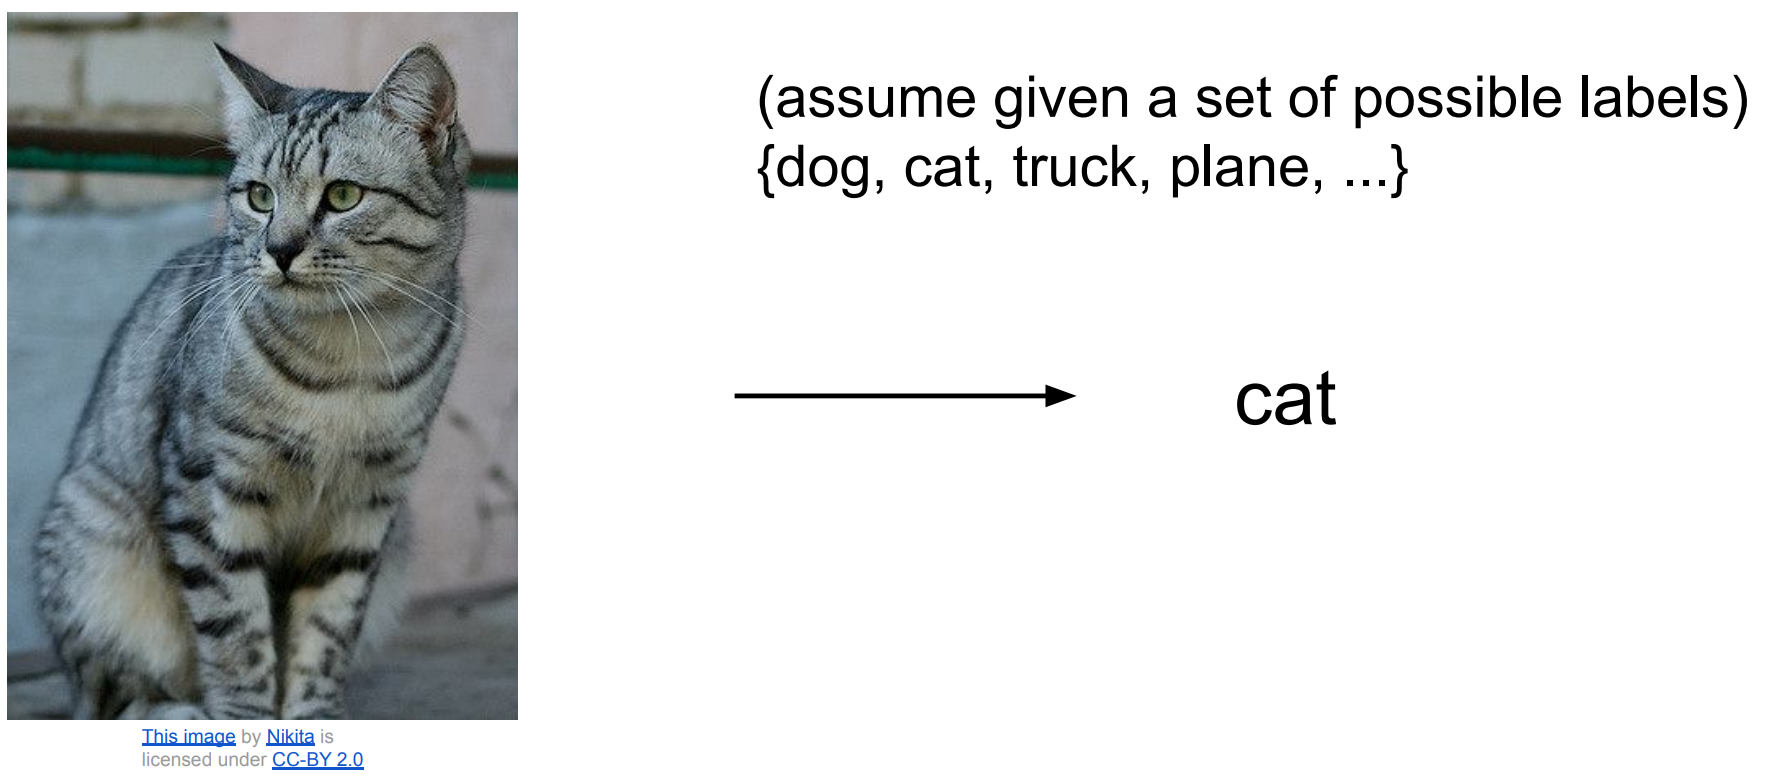
\includegraphics[width=1.0\textwidth,height=0.7\textheight,keepaspectratio]{./images/classification.png}
\end{figure}
    
\end{frame}

\begin{frame}{Computer Vision Tasks}
\begin{figure}
\centering
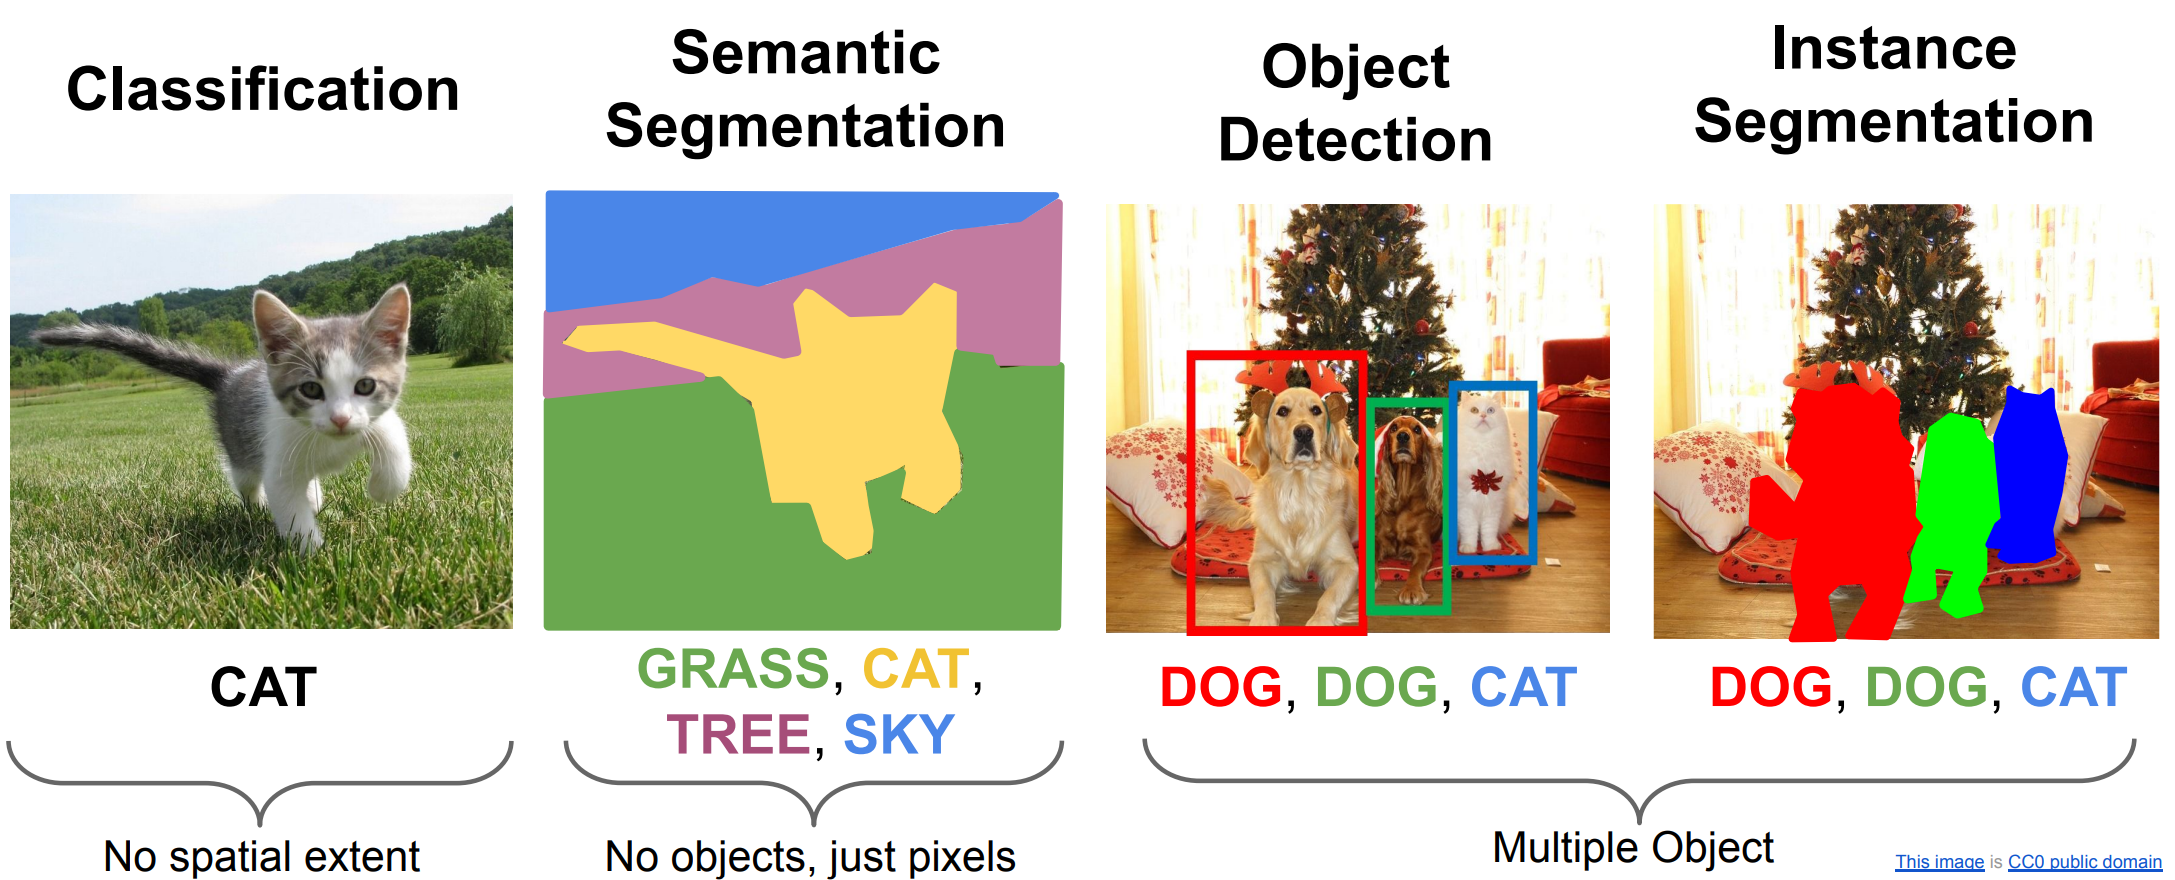
\includegraphics[width=1.0\textwidth,height=1.0\textheight,keepaspectratio]{./images/tasks.png}
\end{figure}
    
\end{frame}

\begin{frame}{Semantic Segmentation}
\begin{figure}
\centering
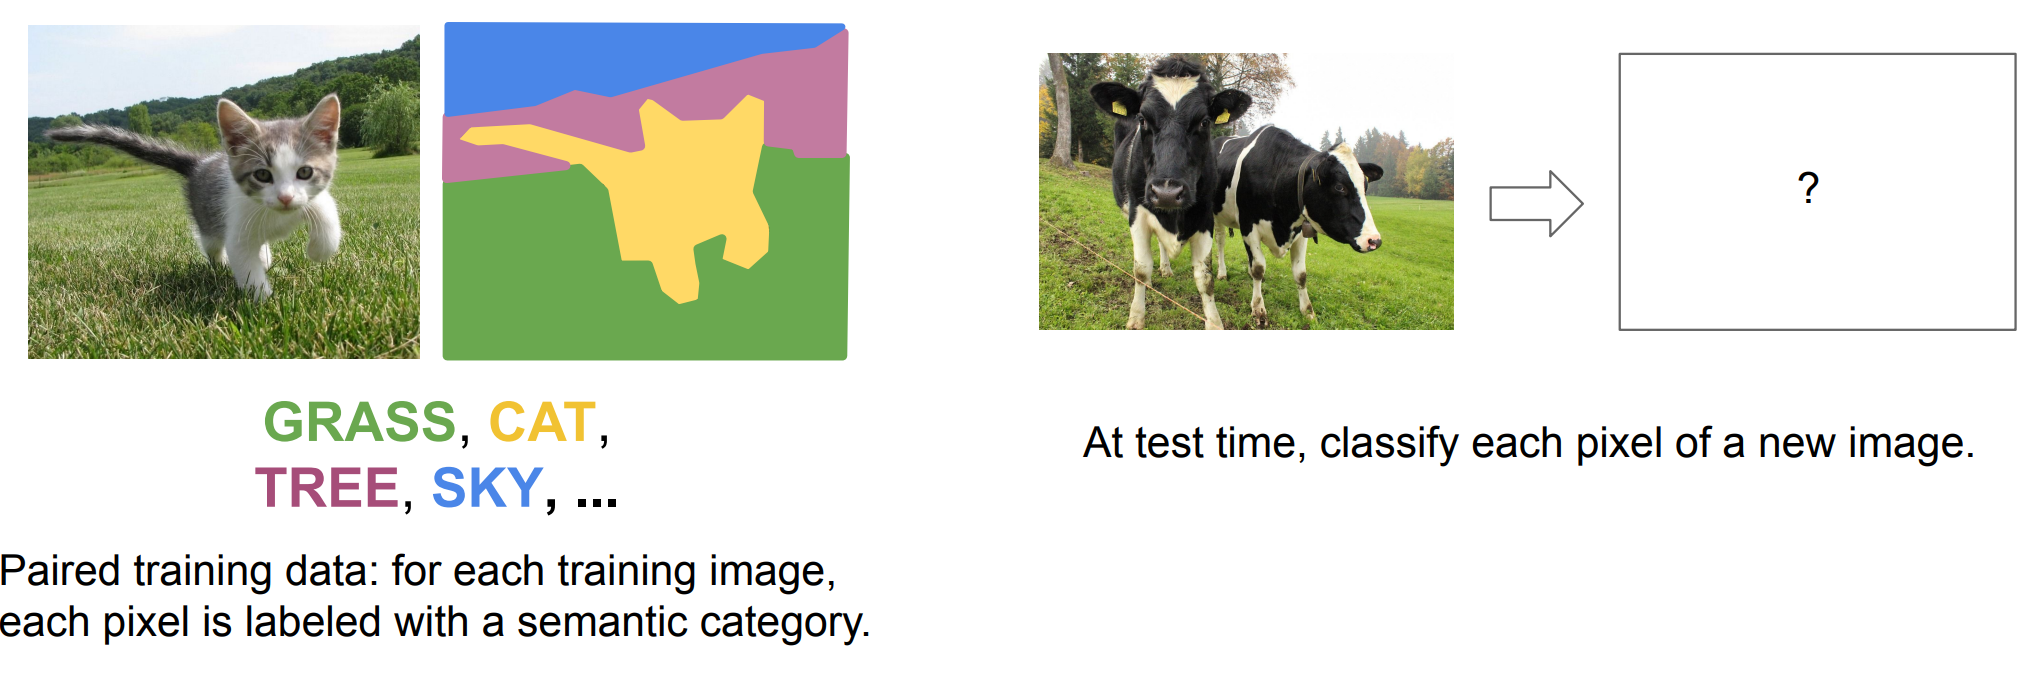
\includegraphics[width=1.0\textwidth,height=1.0\textheight,keepaspectratio]{./images/sem_1.png}
\end{figure}
    
\end{frame}

\begin{frame}{Semantic Segmentation}
\begin{figure}
\centering
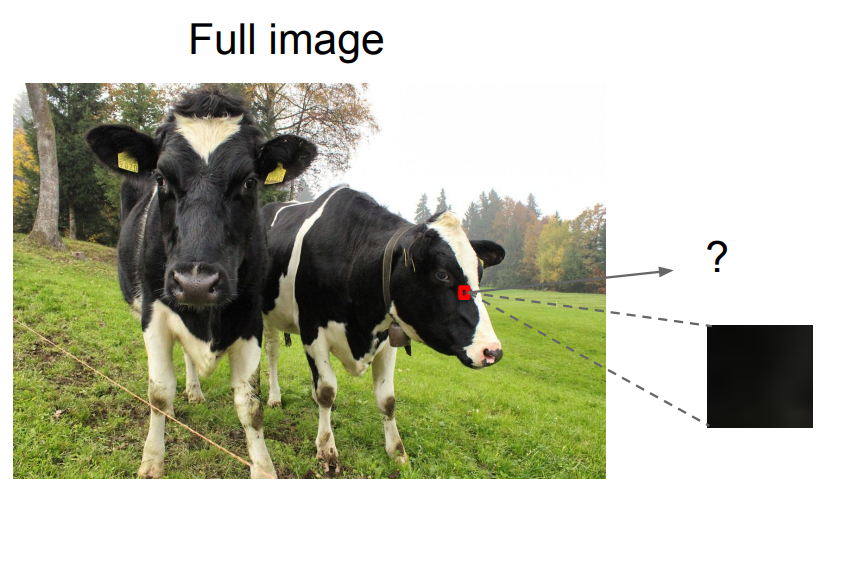
\includegraphics[width=1.0\textwidth,height=0.7\textheight,keepaspectratio]{./images/sem_2.png}
\end{figure}
\pause

\begin{itemize}
    \item Impossible to classify without context
    \item How do we include context?
\end{itemize}
\end{frame}

\begin{frame}[allowframebreaks]{Semantic Segmentation Idea: Sliding Window}
\begin{figure}
\centering
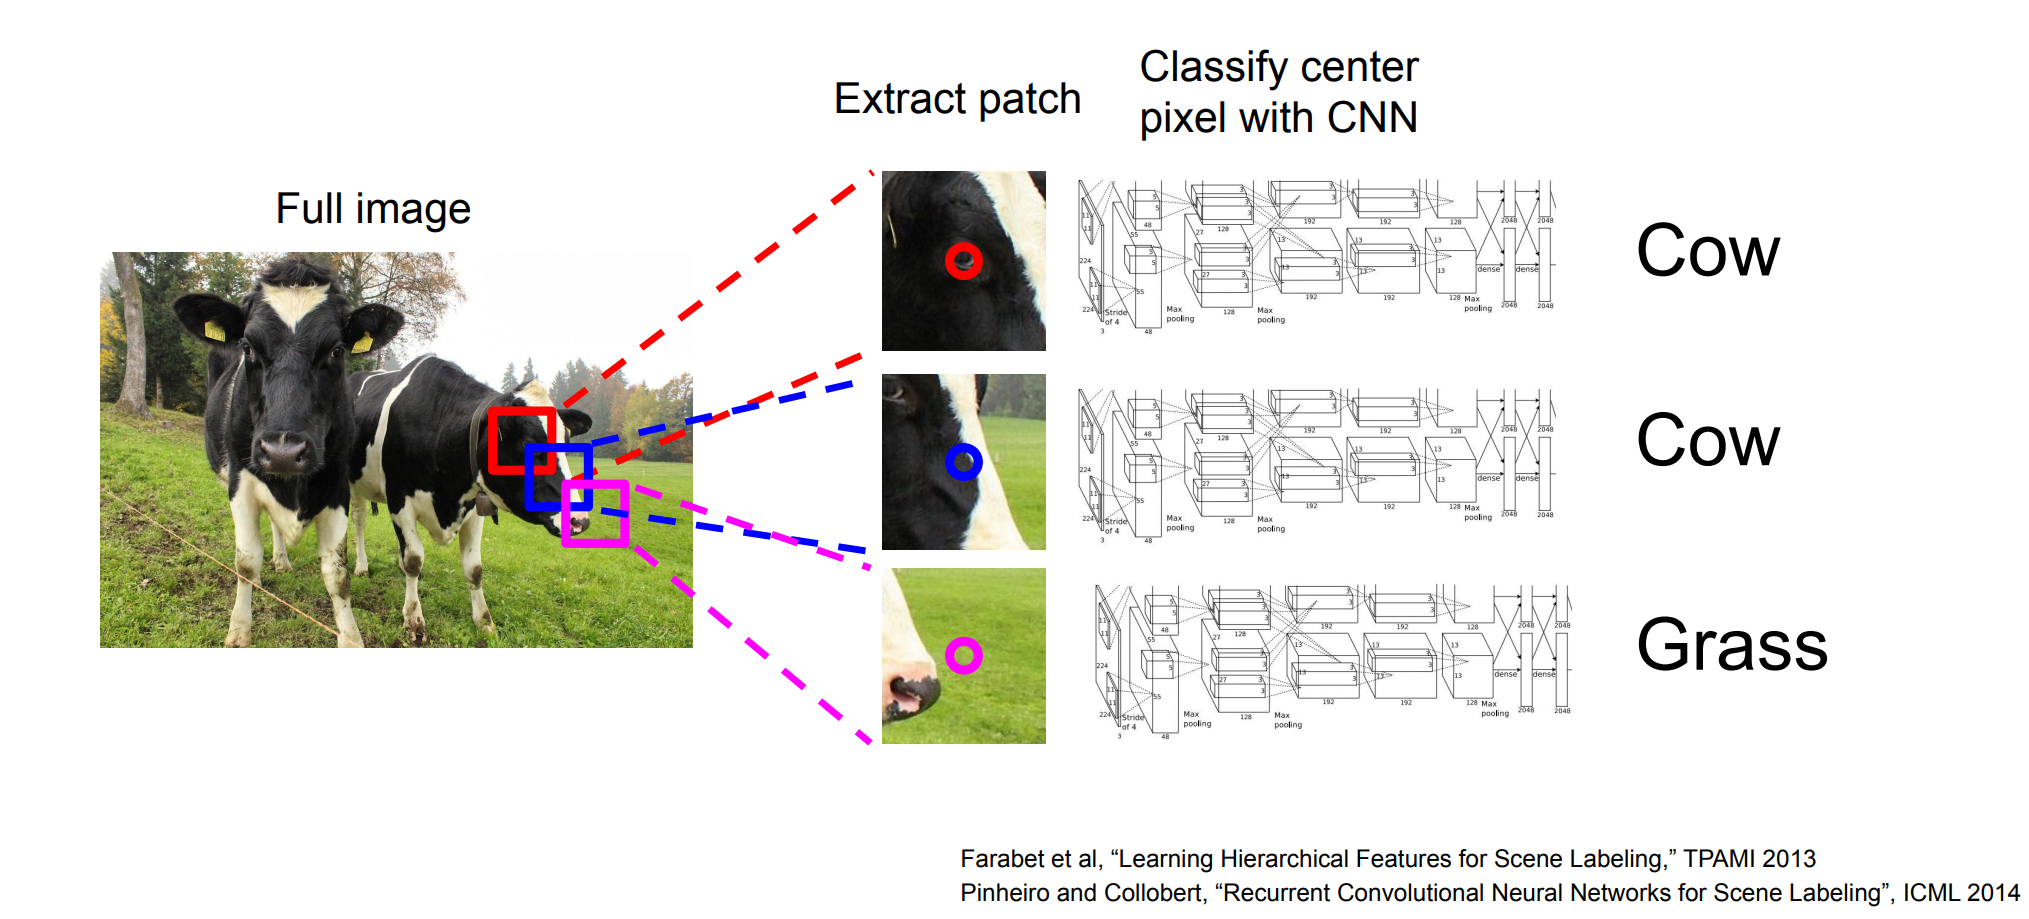
\includegraphics[width=1.0\textwidth,height=1.0\textheight,keepaspectratio]{./images/sem_3.png}
\end{figure}

\framebreak

\begin{figure}
\centering
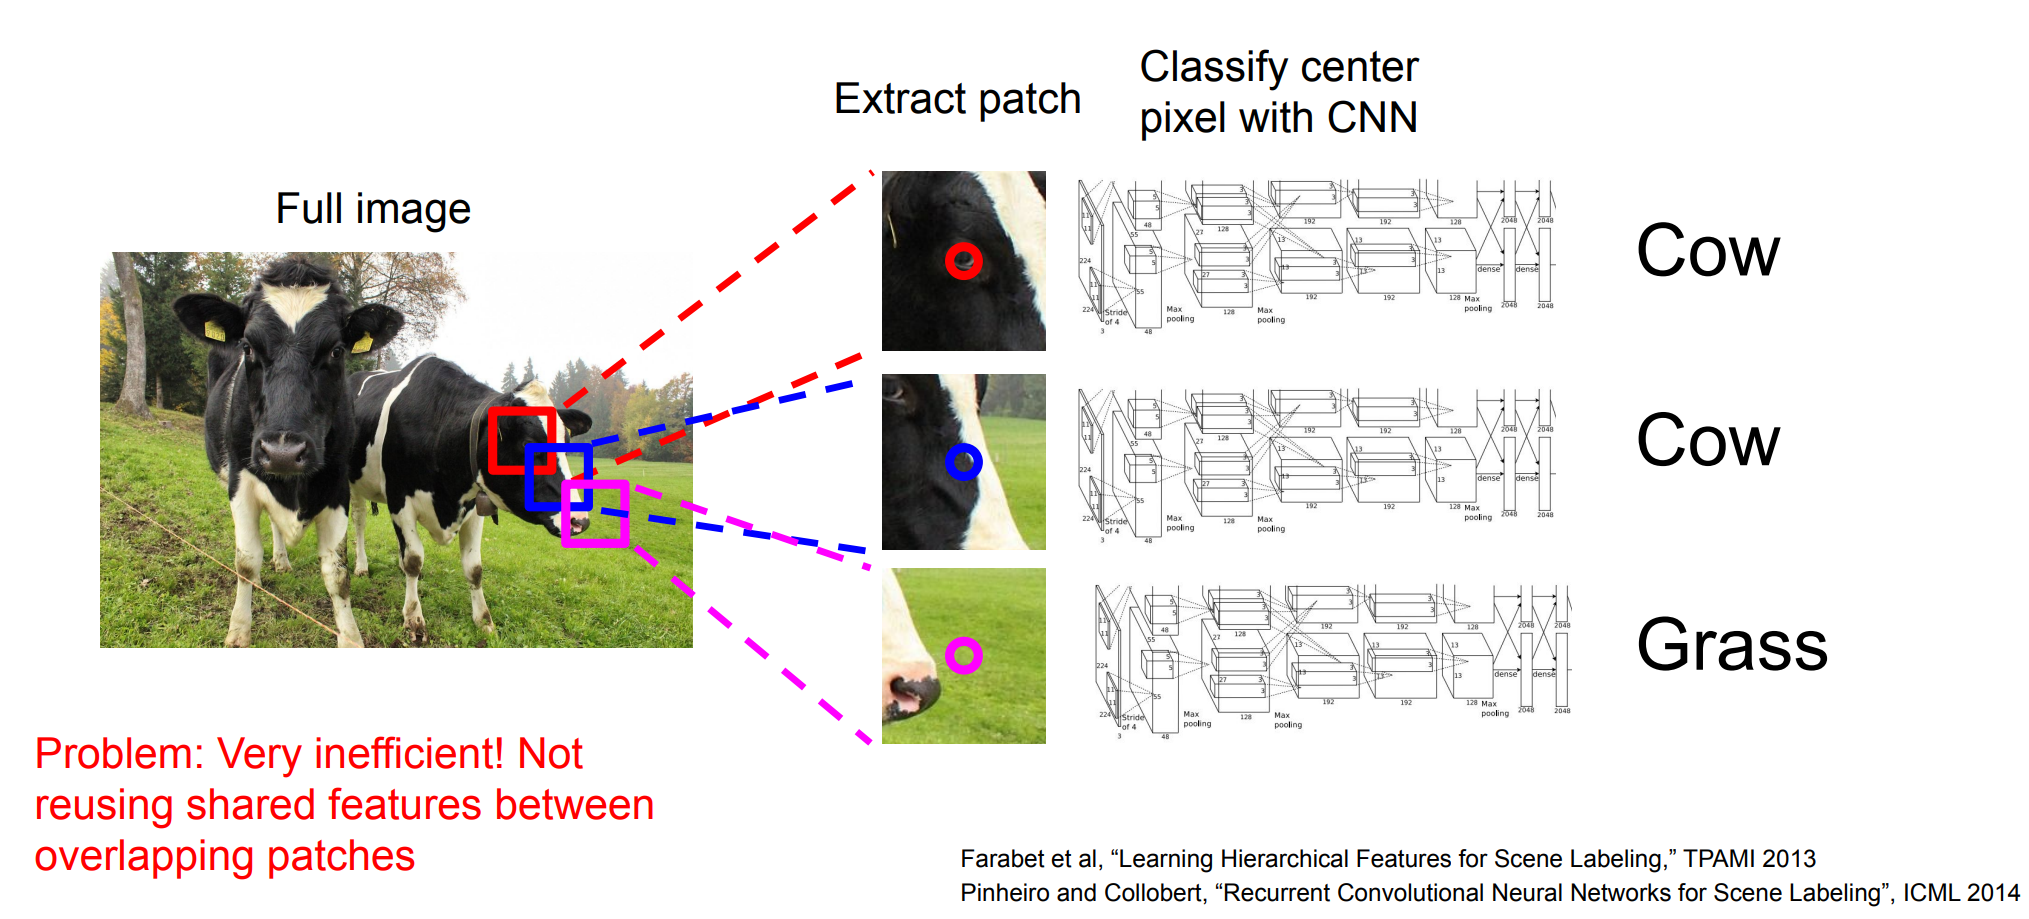
\includegraphics[width=1.0\textwidth,height=1.0\textheight,keepaspectratio]{./images/sem_4.png}
\end{figure}
    
\end{frame}

\begin{frame}[allowframebreaks]{Semantic Segmentation Idea: Convolution}
\begin{figure}
\centering
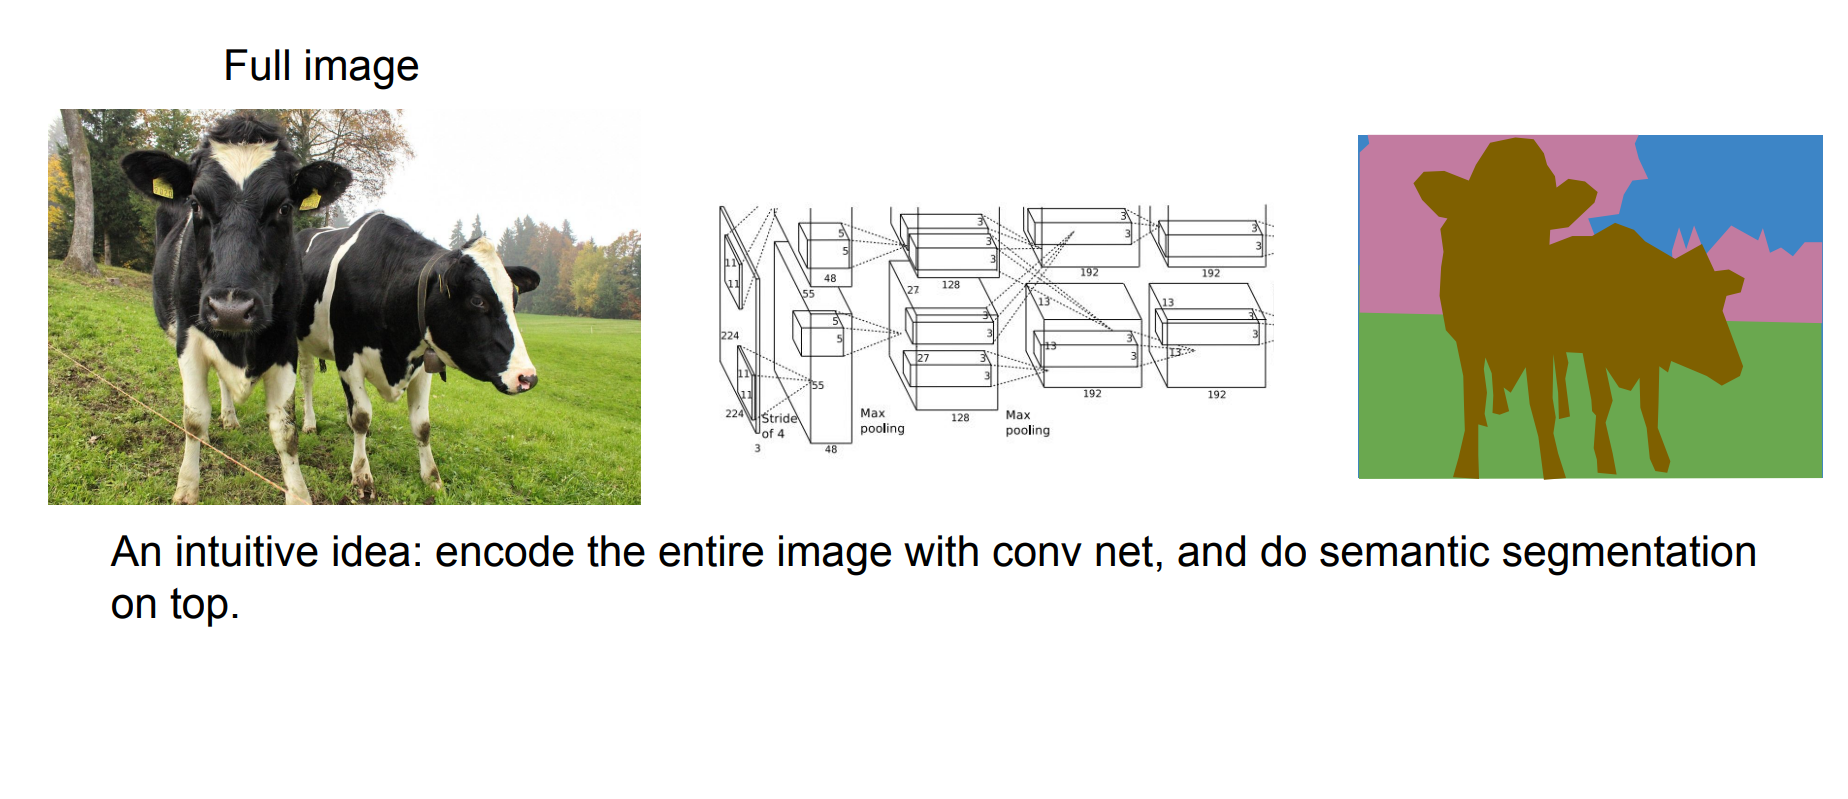
\includegraphics[width=1.0\textwidth,height=1.0\textheight,keepaspectratio]{./images/sem_5.png}
\end{figure}

\framebreak

\begin{figure}
\centering
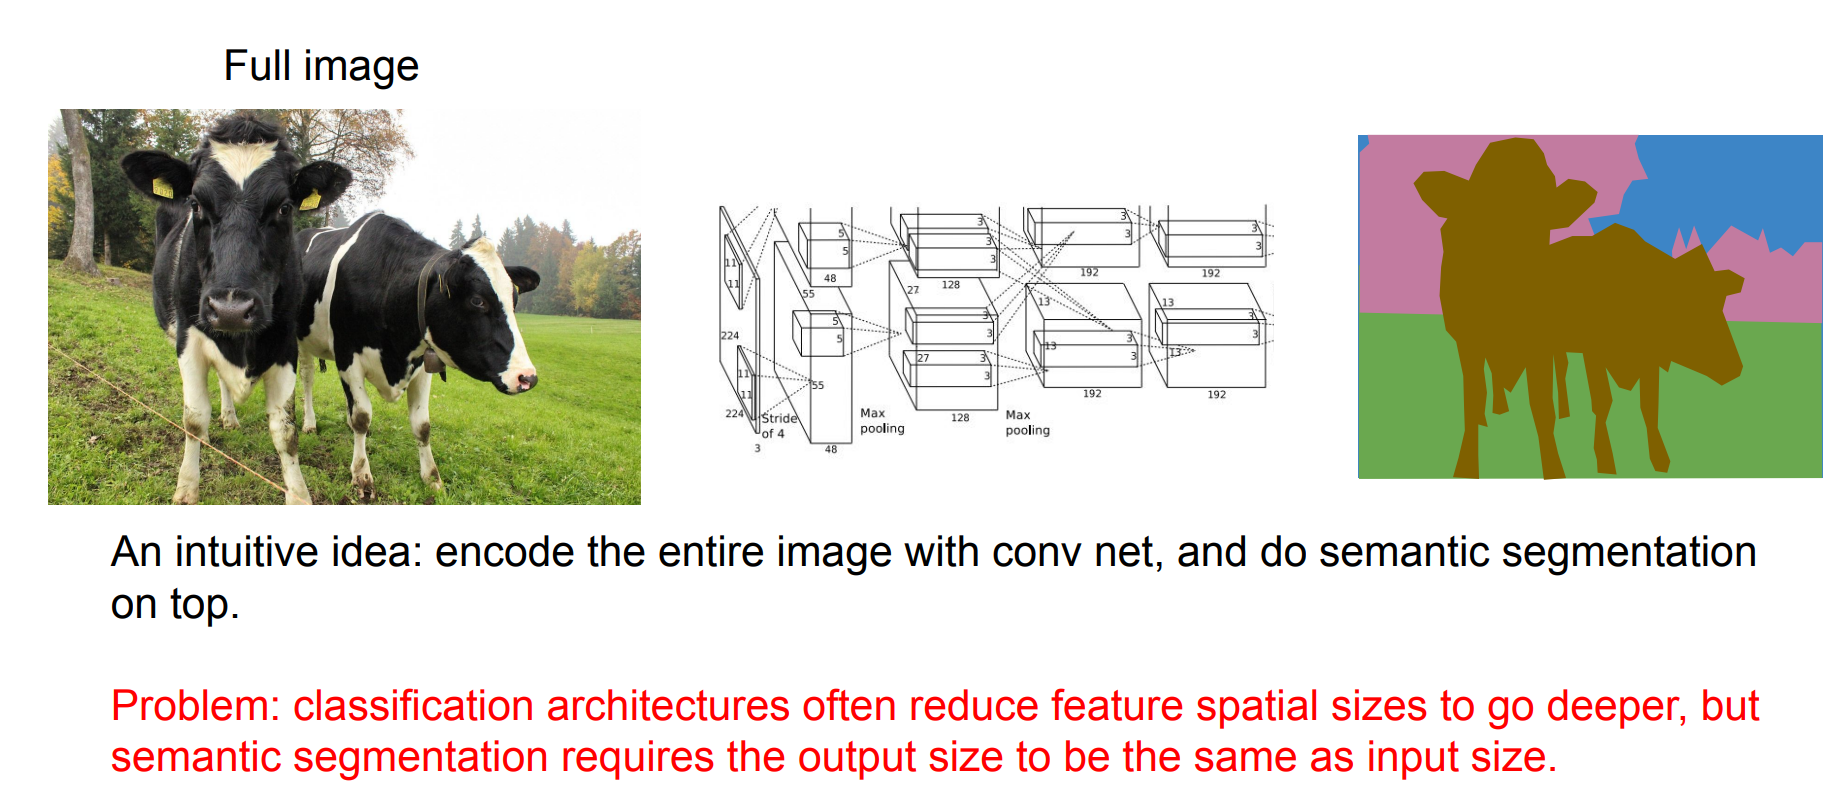
\includegraphics[width=1.0\textwidth,height=1.0\textheight,keepaspectratio]{./images/sem_6.png}
\end{figure}
    
\end{frame}

\begin{frame}[allowframebreaks]{Semantic Segmentation Idea: Fully Convolutional}
\begin{figure}
\centering
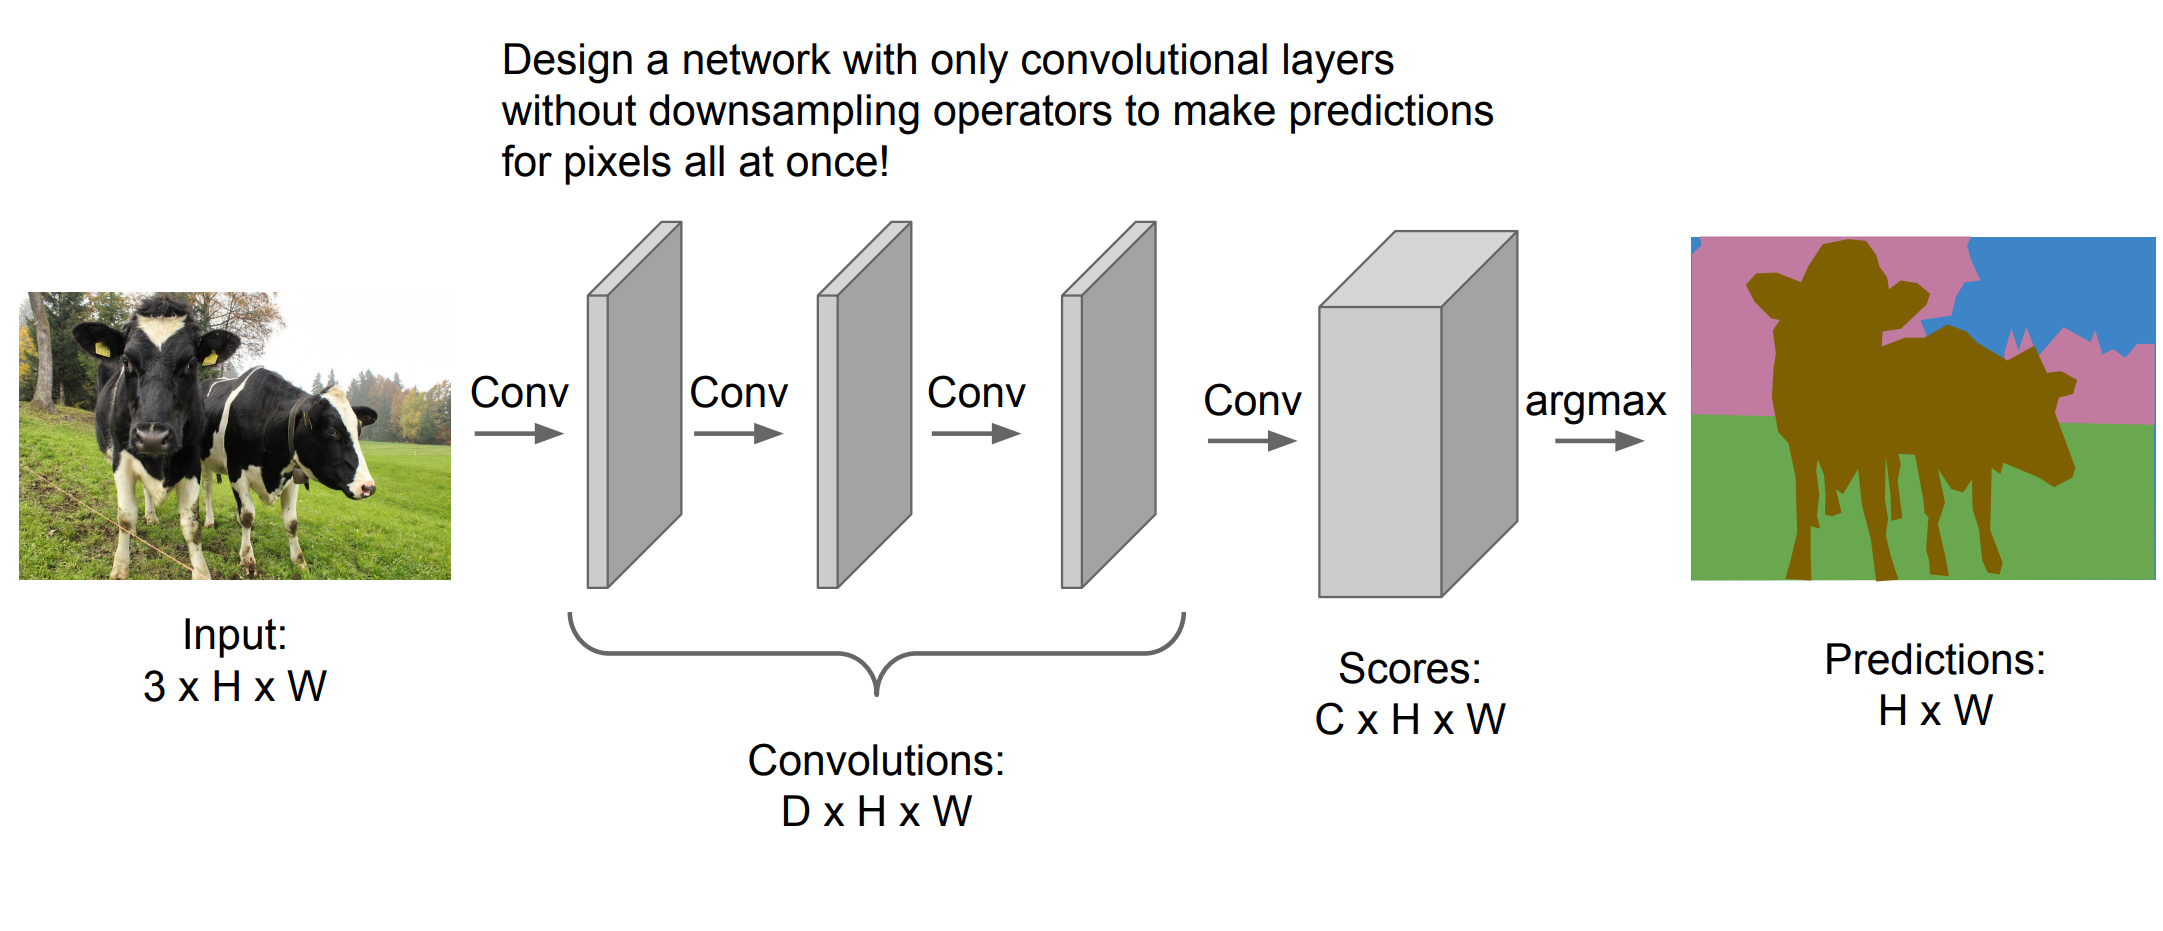
\includegraphics[width=1.0\textwidth,height=1.0\textheight,keepaspectratio]{./images/sem_7.png}
\end{figure}

\framebreak

\begin{figure}
\centering
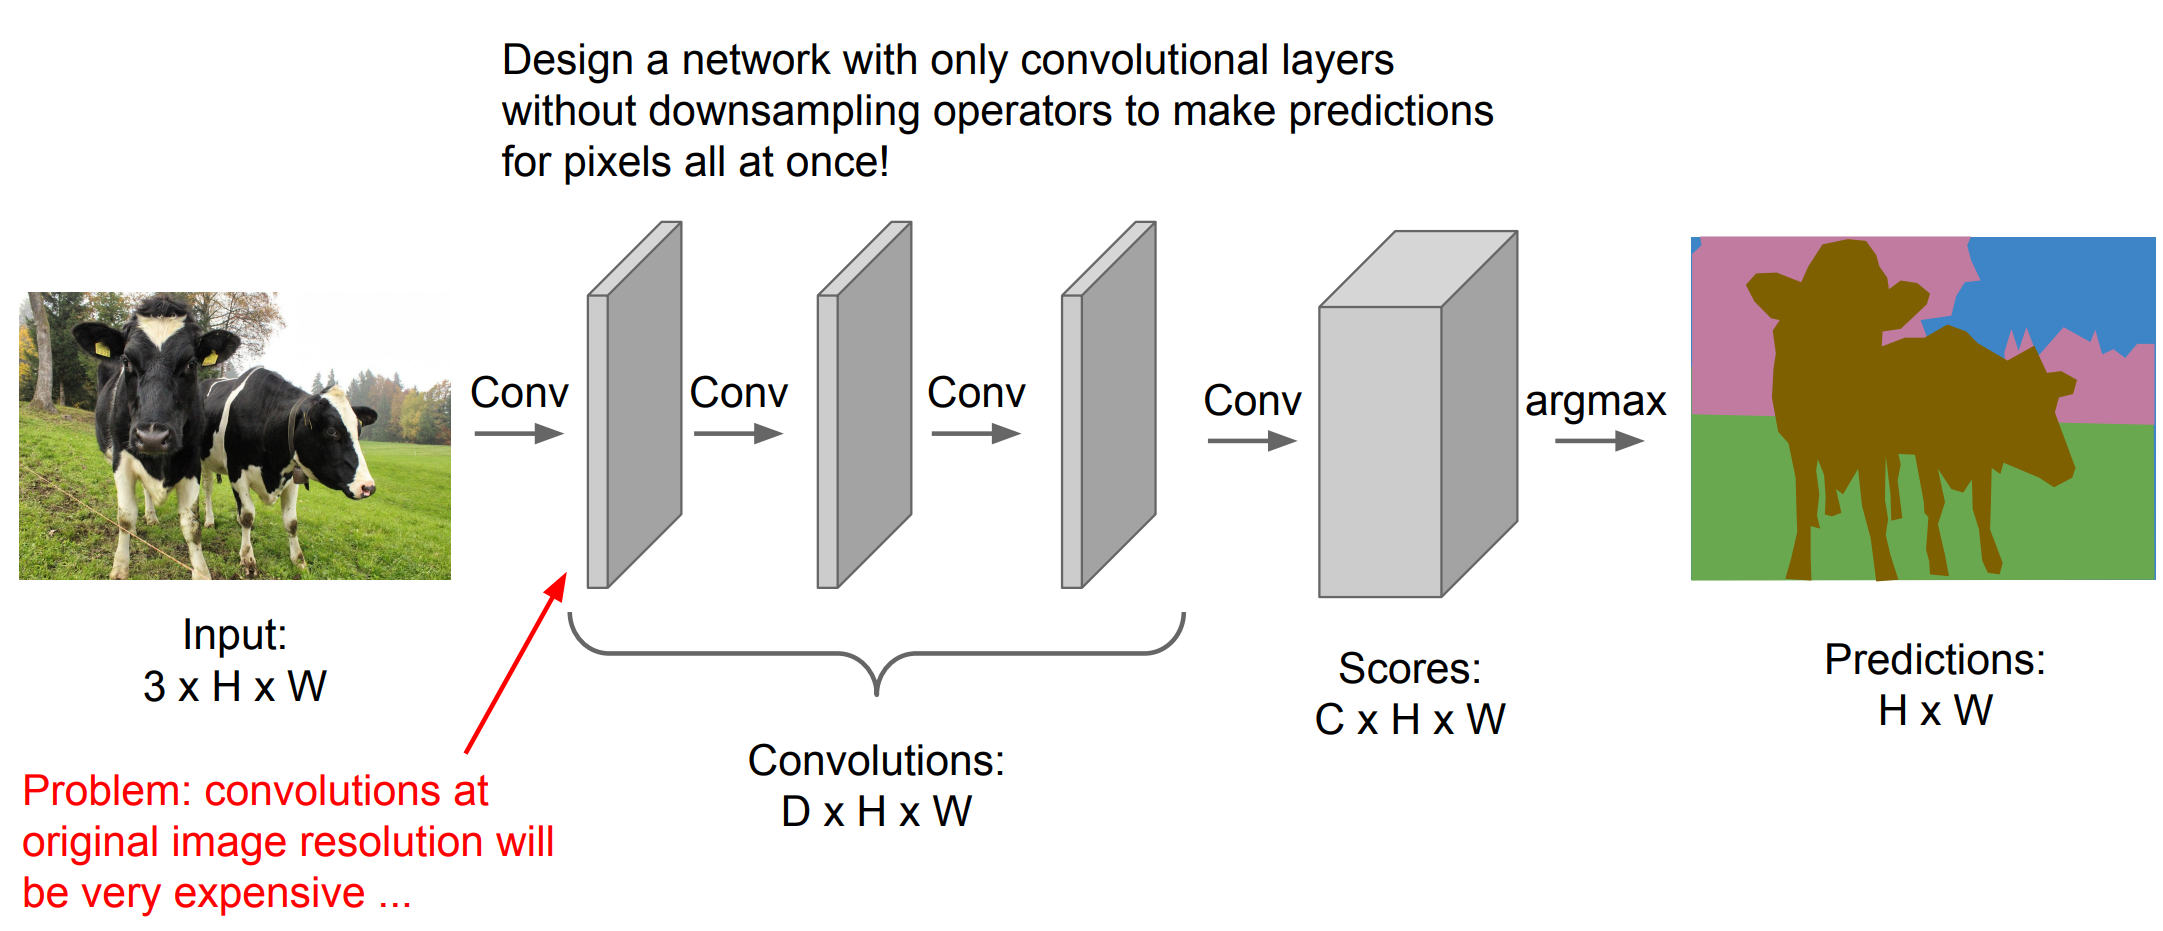
\includegraphics[width=1.0\textwidth,height=1.0\textheight,keepaspectratio]{./images/sem_8.png}
\end{figure}

\framebreak

\begin{figure}
\centering
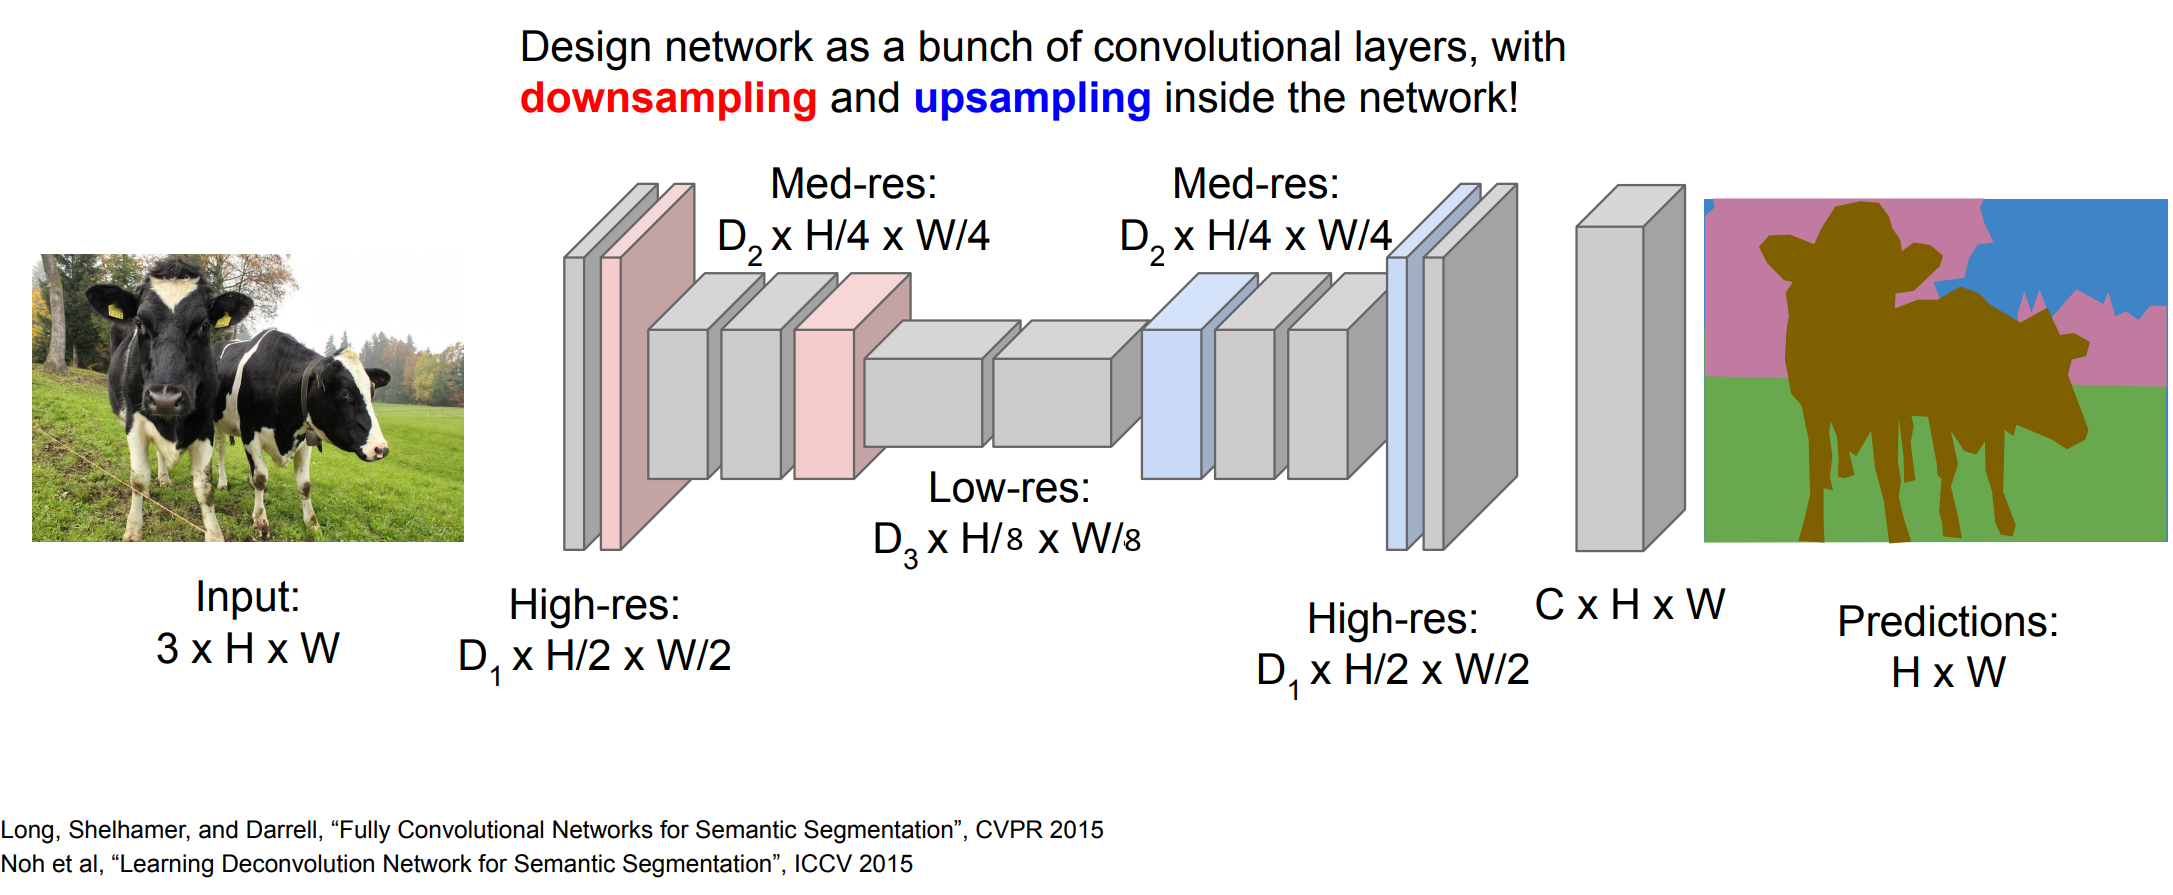
\includegraphics[width=1.0\textwidth,height=1.0\textheight,keepaspectratio]{./images/sem_9.png}
\end{figure}

\framebreak

\begin{figure}
\centering
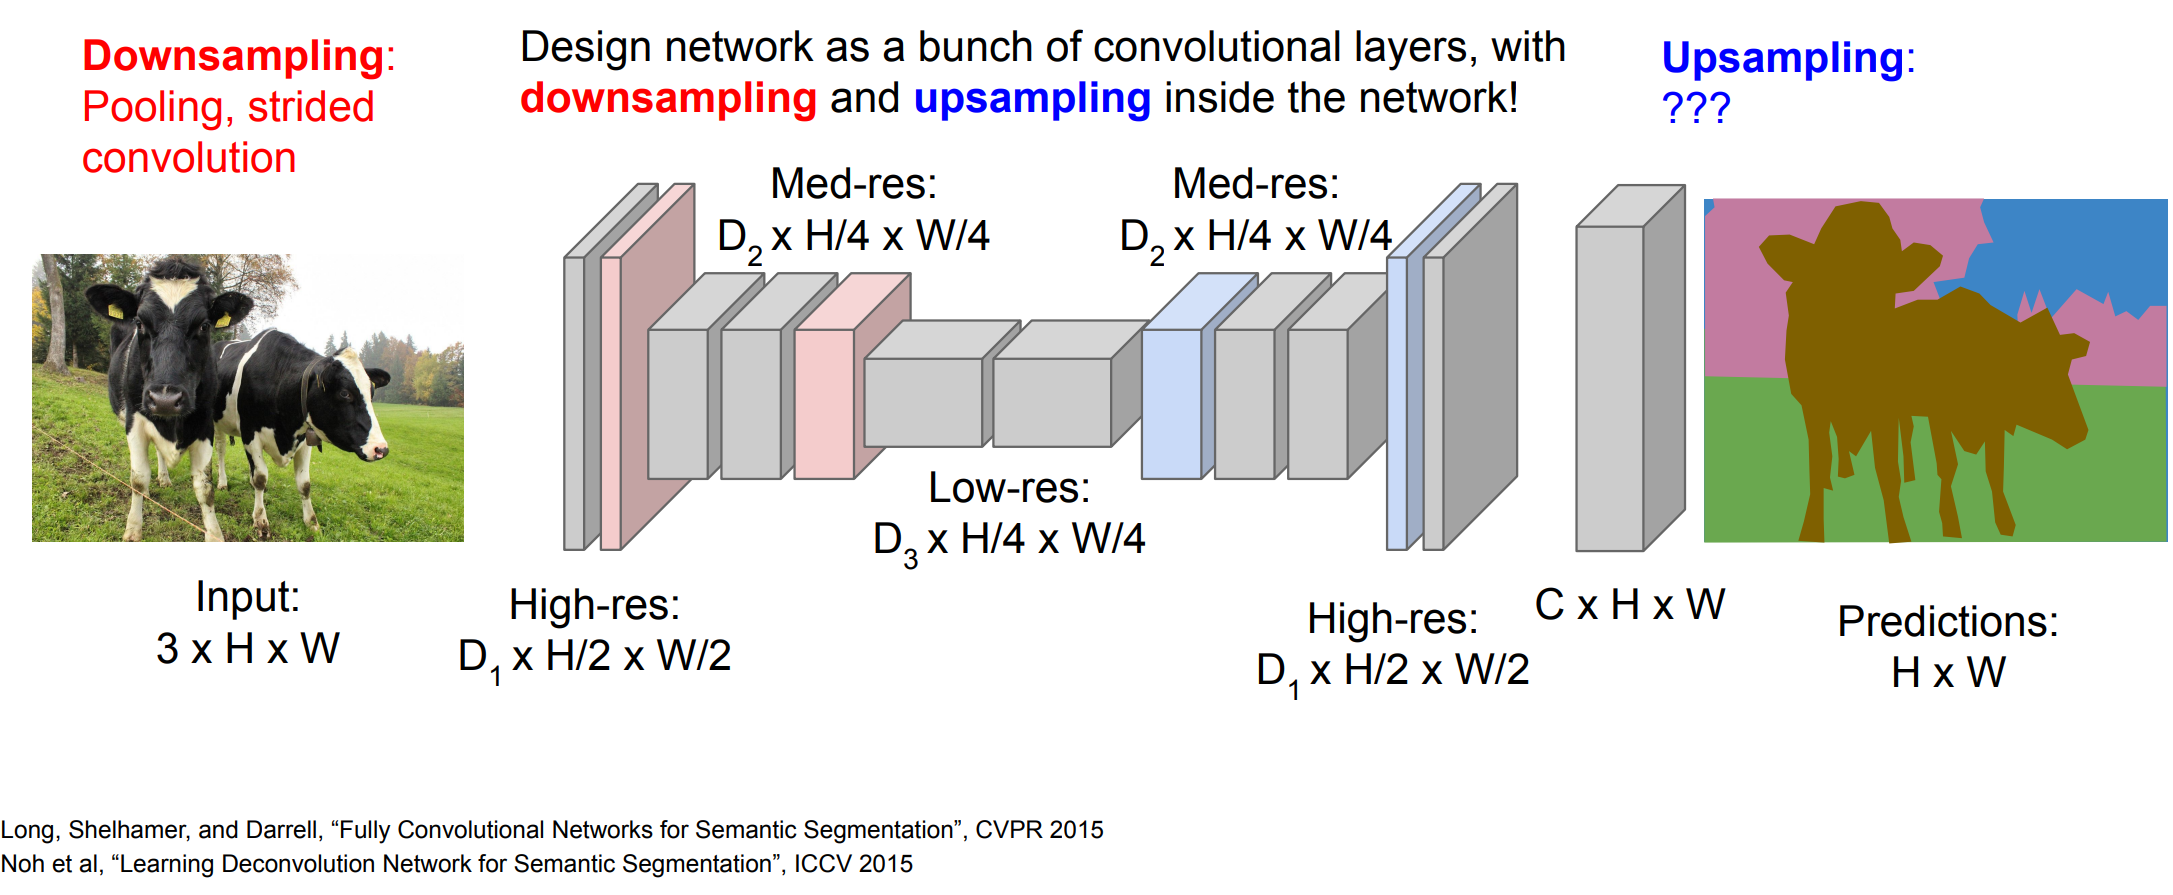
\includegraphics[width=1.0\textwidth,height=1.0\textheight,keepaspectratio]{./images/sem_10.png}
\end{figure}
    
\end{frame}

\begin{frame}{In-Network Upsampling: Unpooling}
\begin{figure}
\centering
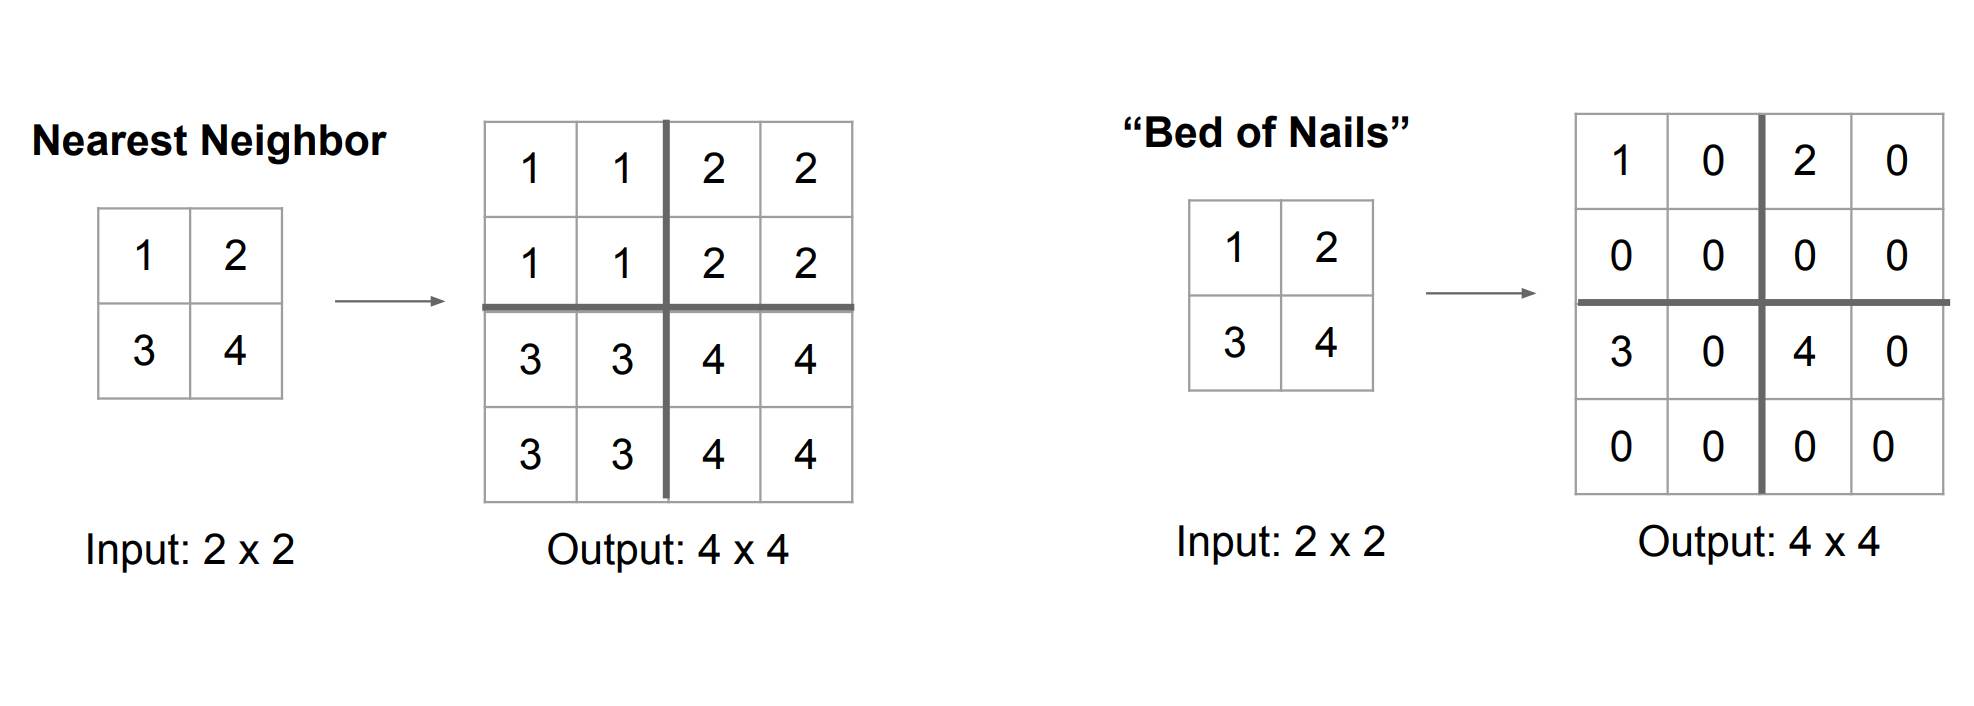
\includegraphics[width=1.0\textwidth,height=1.0\textheight,keepaspectratio]{./images/upsample_1.png}
\end{figure}

\end{frame}

\begin{frame}{In-Network Upsampling: Max Unpooling}
\begin{figure}
\centering
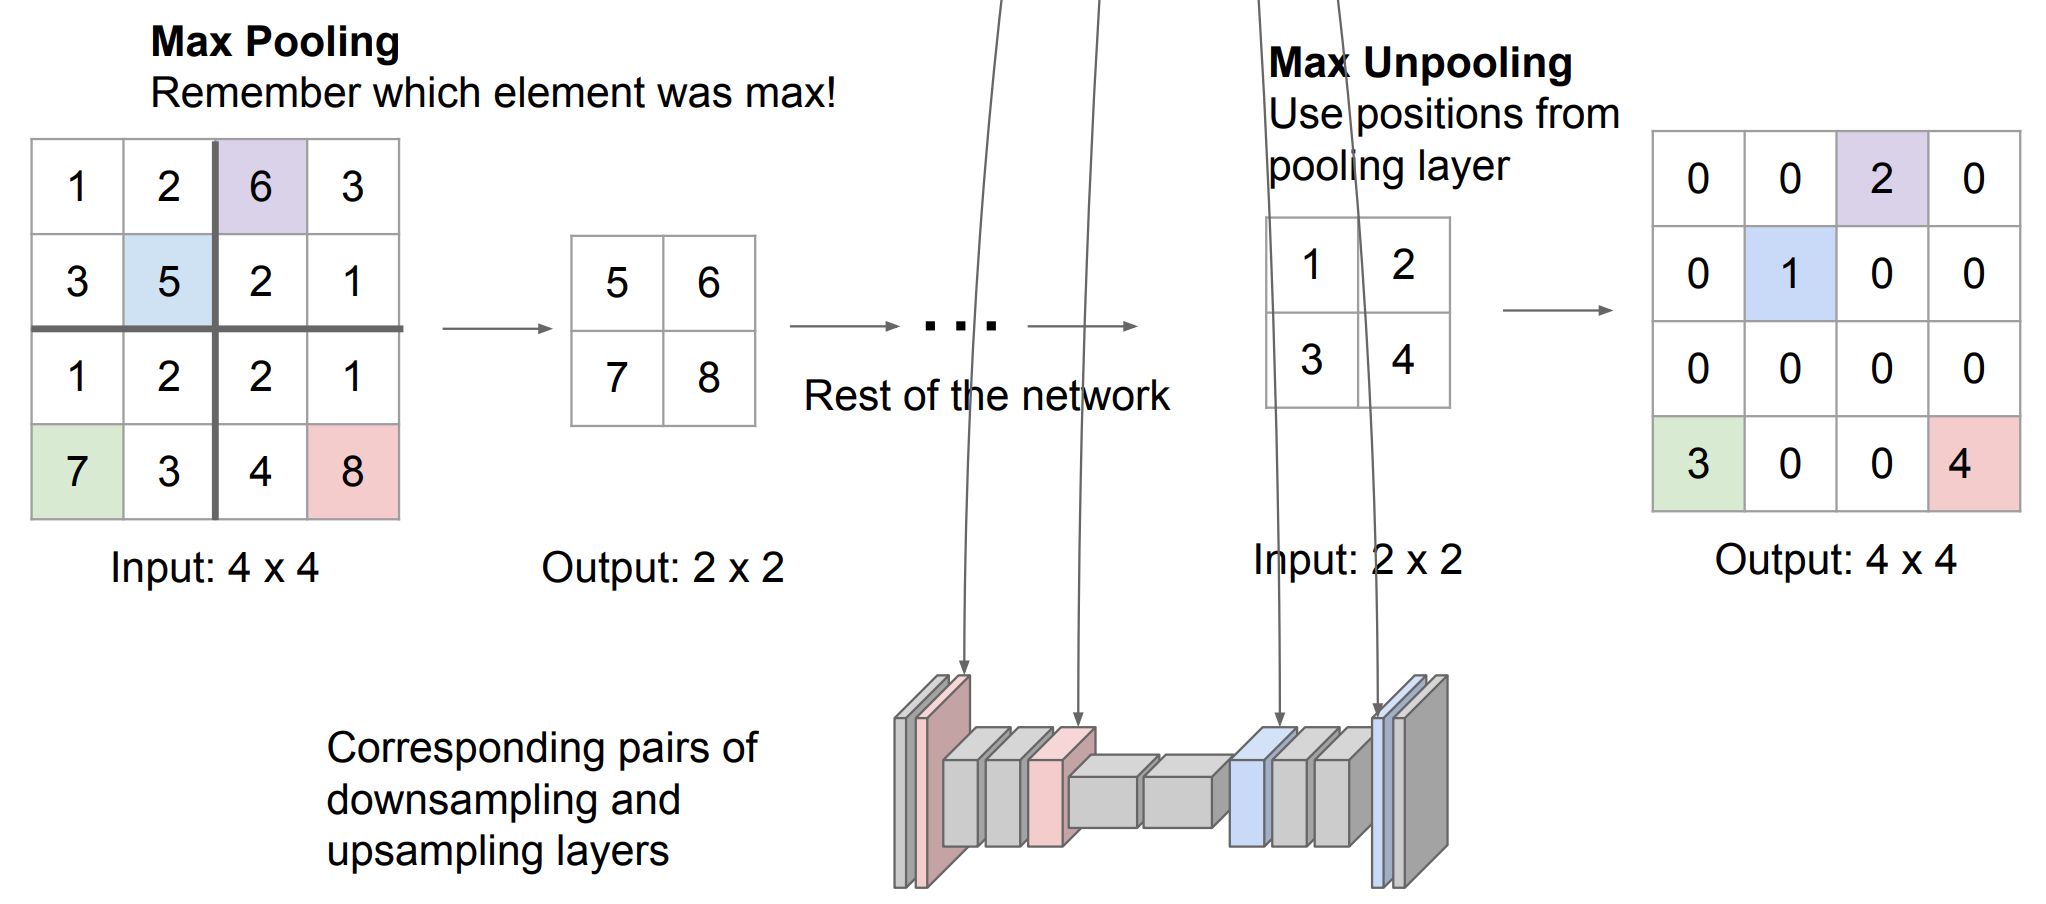
\includegraphics[width=1.0\textwidth,height=1.0\textheight,keepaspectratio]{./images/upsample_2.png}
\end{figure}

\end{frame}

\begin{frame}[allowframebreaks]{Learnable Upsampling: Transposed Convolution}
\begin{figure}
\centering
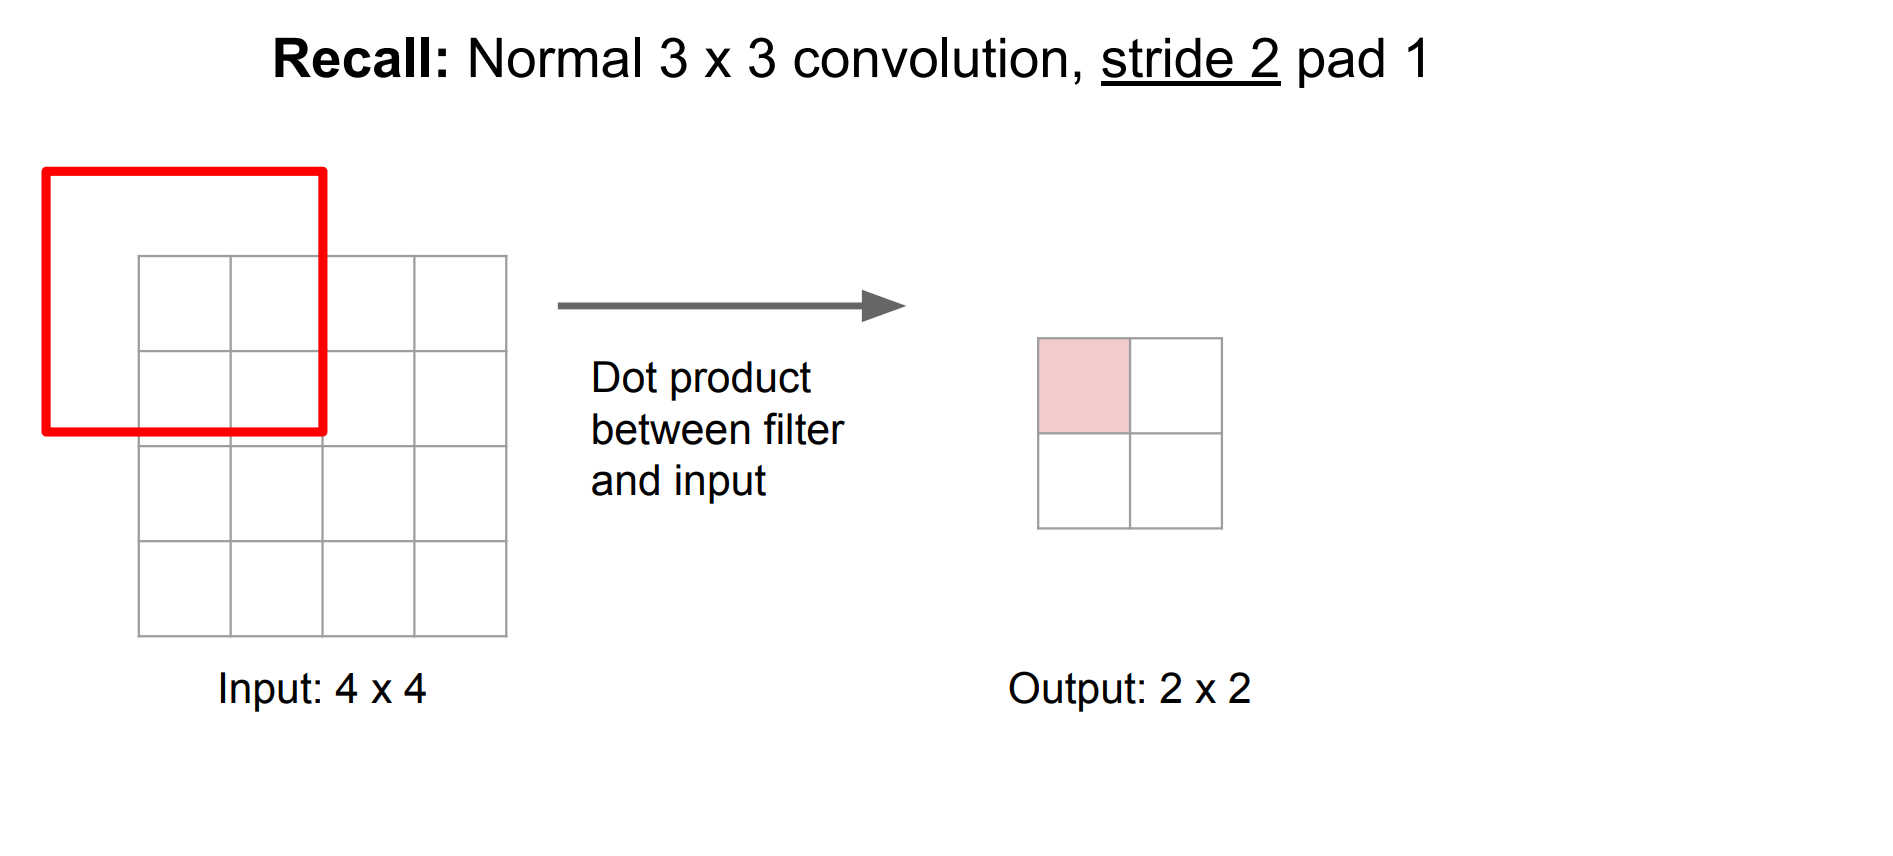
\includegraphics[width=1.0\textwidth,height=1.0\textheight,keepaspectratio]{./images/upsample_3.png}
\end{figure}

\framebreak

\begin{figure}
\centering
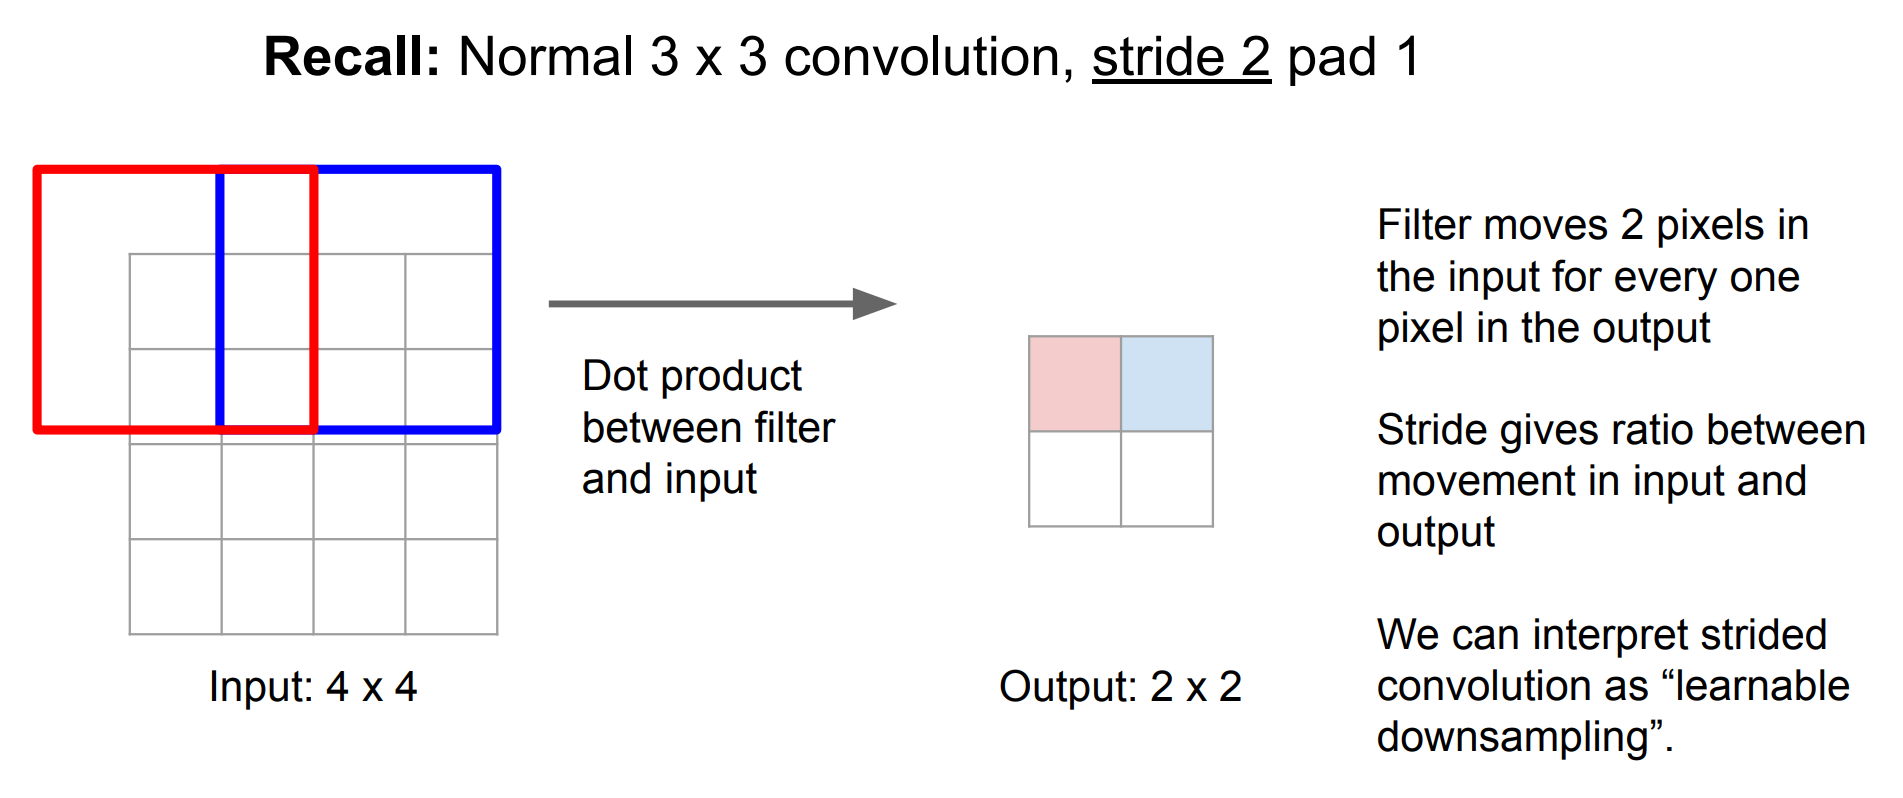
\includegraphics[width=1.0\textwidth,height=1.0\textheight,keepaspectratio]{./images/upsample_4.png}
\end{figure}

\framebreak

\begin{figure}
\centering
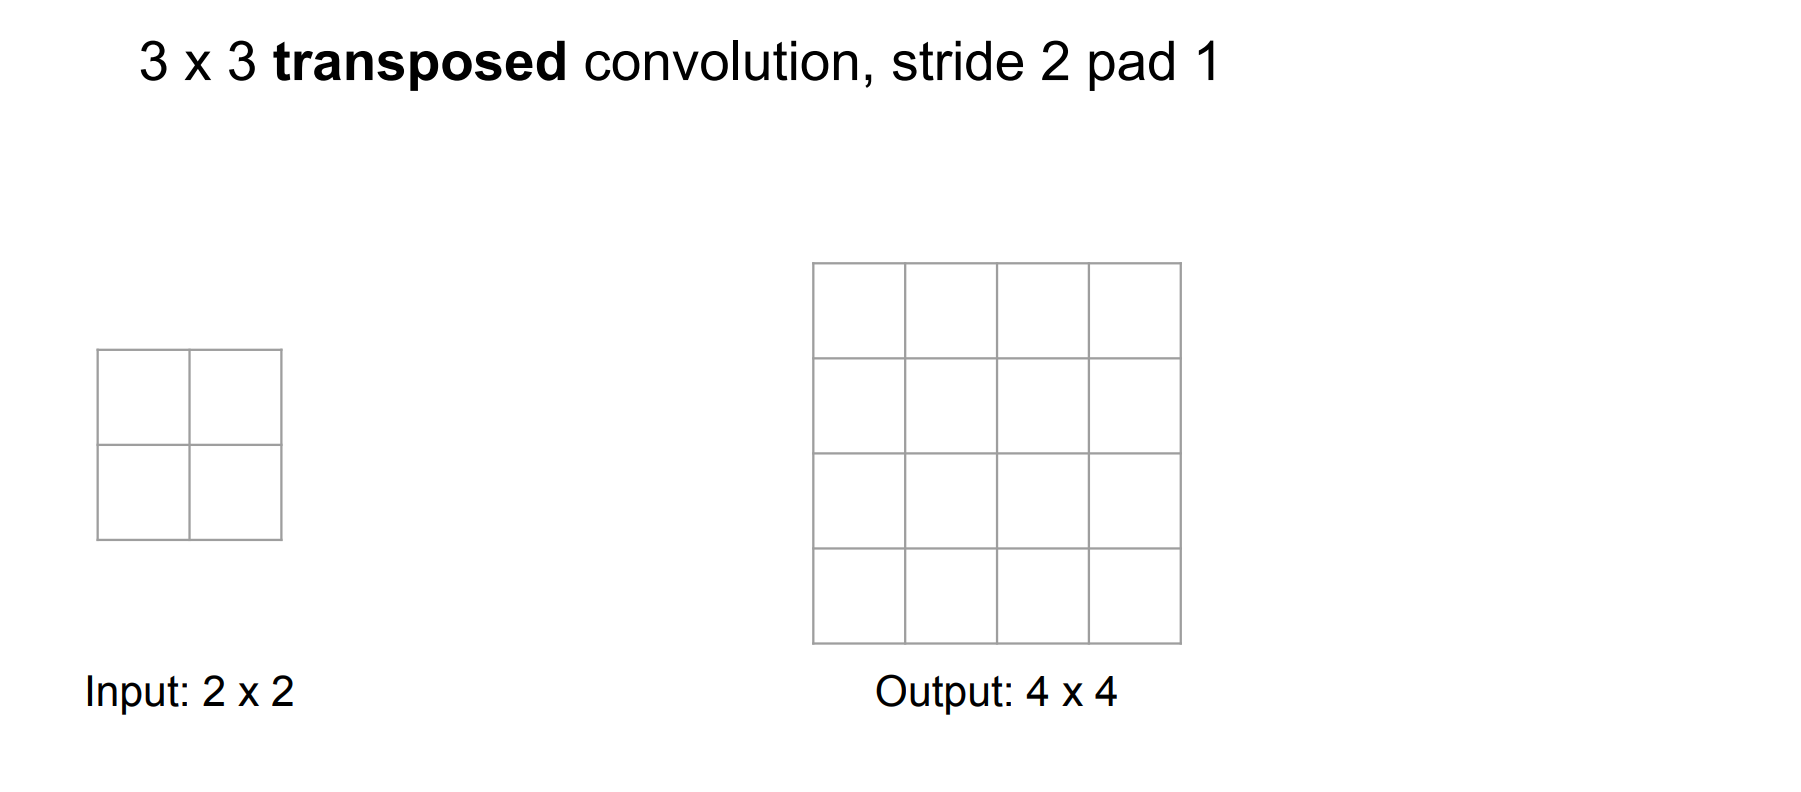
\includegraphics[width=1.0\textwidth,height=1.0\textheight,keepaspectratio]{./images/upsample_5.png}
\end{figure}

\framebreak

\begin{figure}
\centering
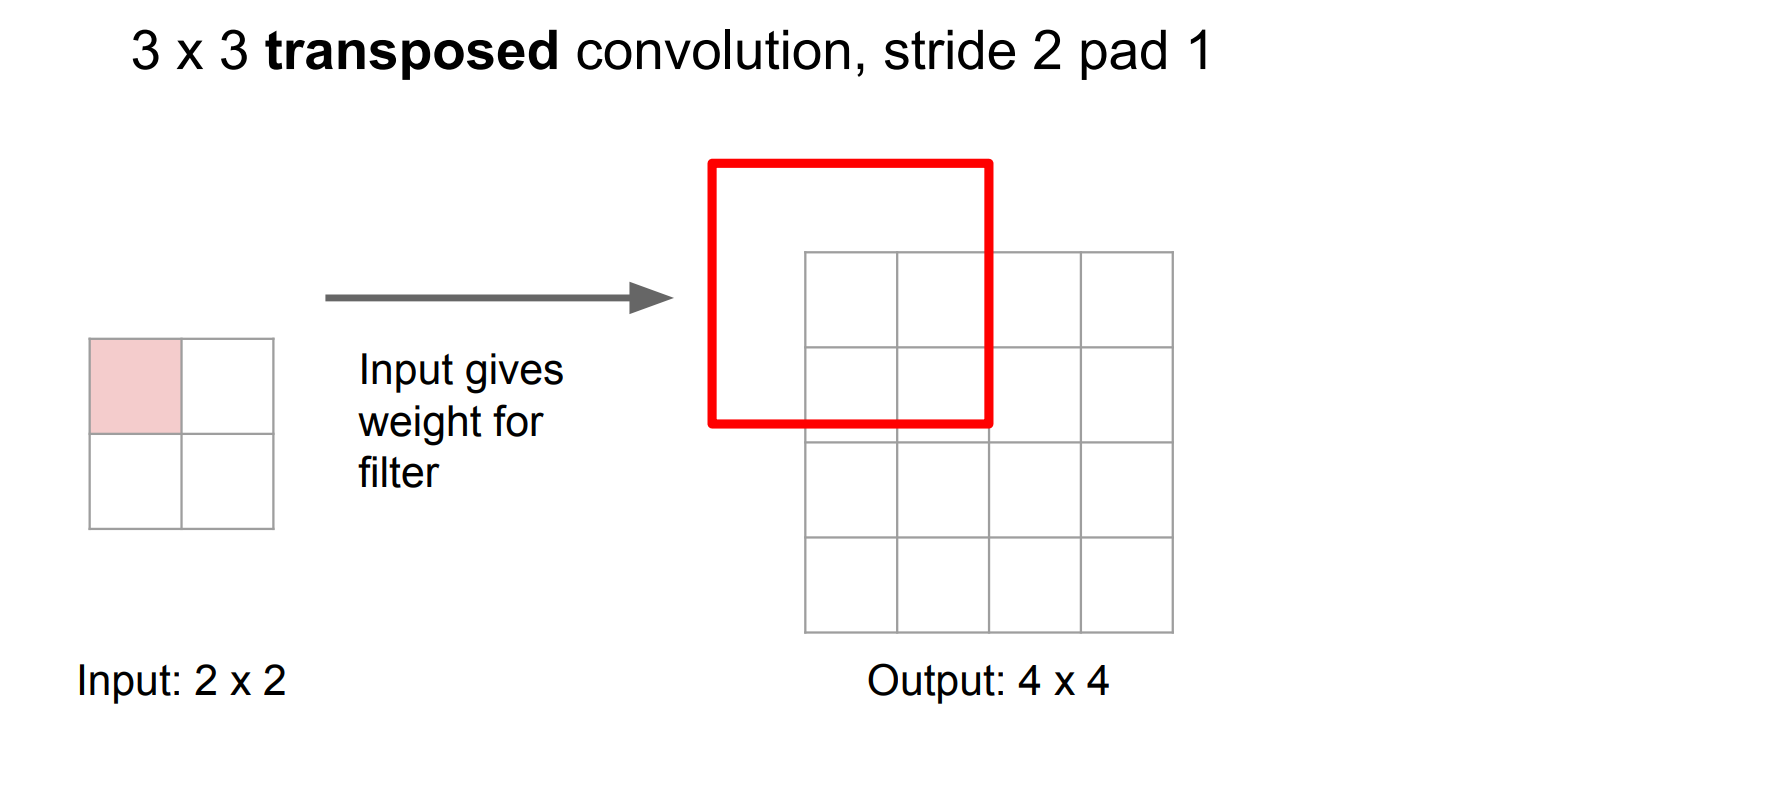
\includegraphics[width=1.0\textwidth,height=1.0\textheight,keepaspectratio]{./images/upsample_6.png}
\end{figure}

\framebreak

\begin{figure}
\centering
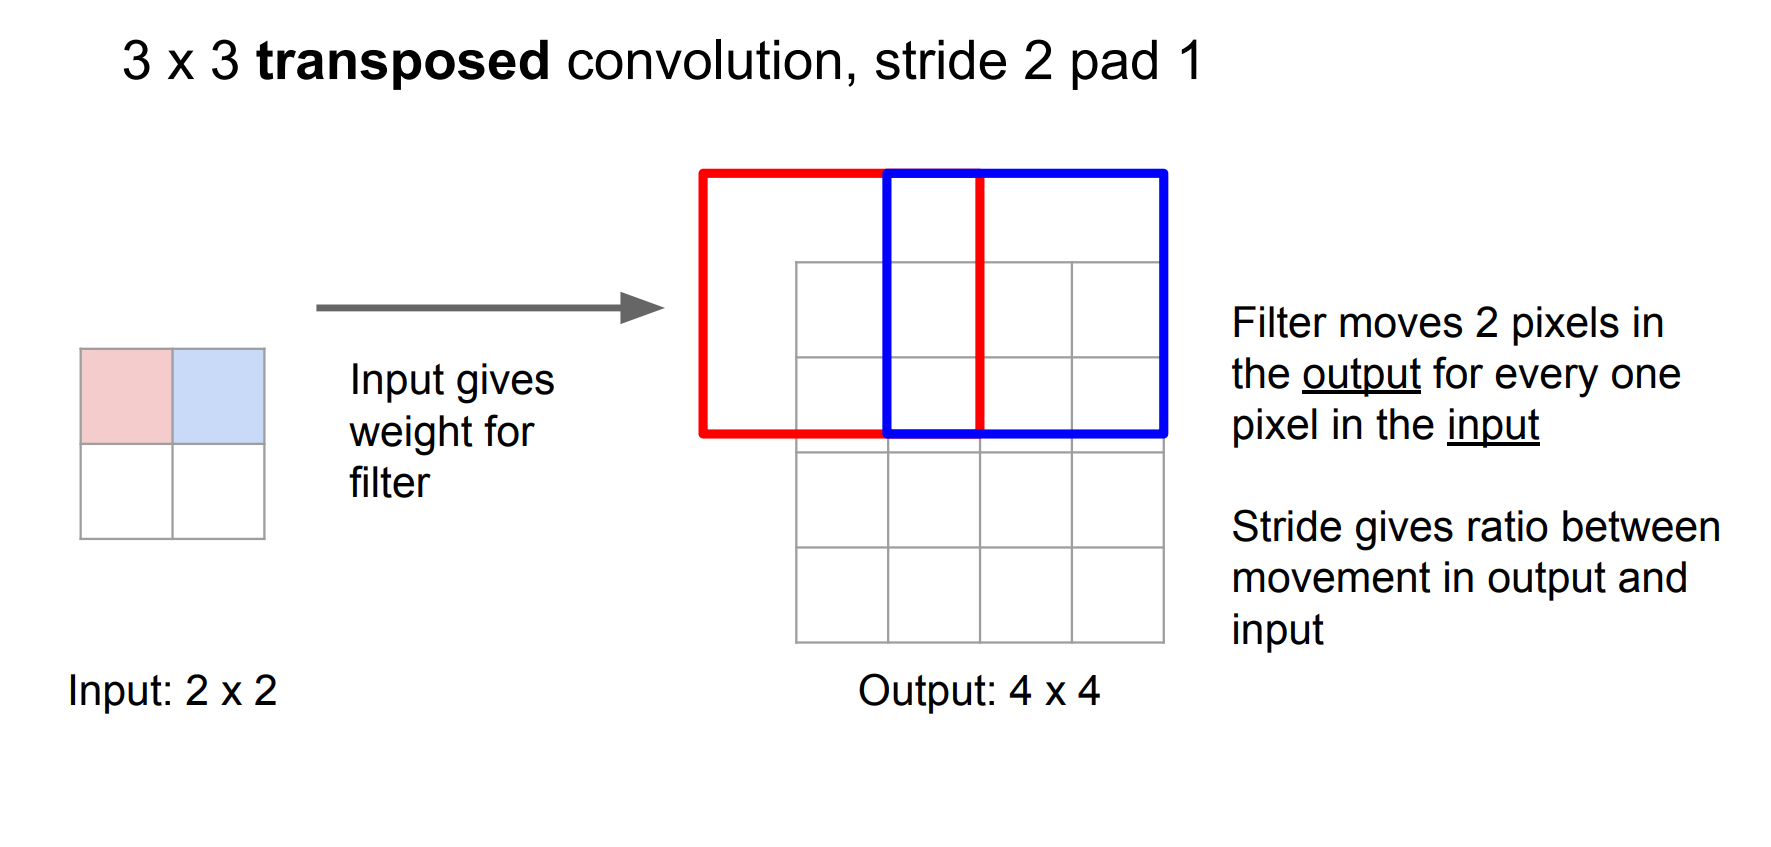
\includegraphics[width=1.0\textwidth,height=1.0\textheight,keepaspectratio]{./images/upsample_7.png}
\end{figure}

\framebreak

\begin{figure}
\centering
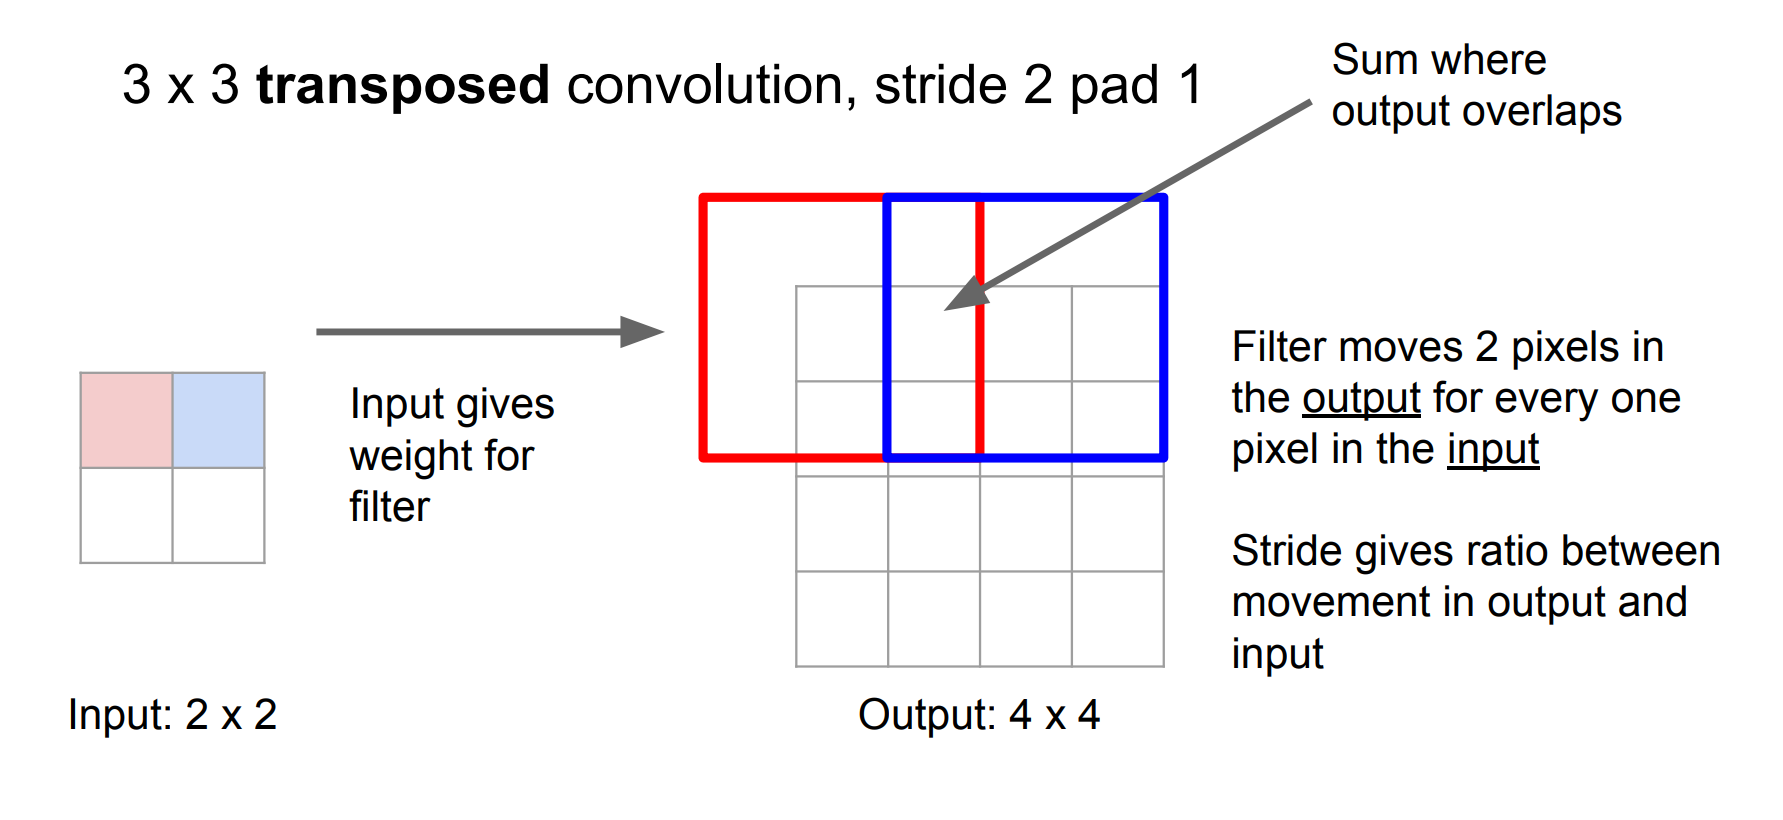
\includegraphics[width=1.0\textwidth,height=1.0\textheight,keepaspectratio]{./images/upsample_8.png}
\end{figure}

\begin{figure}
\centering
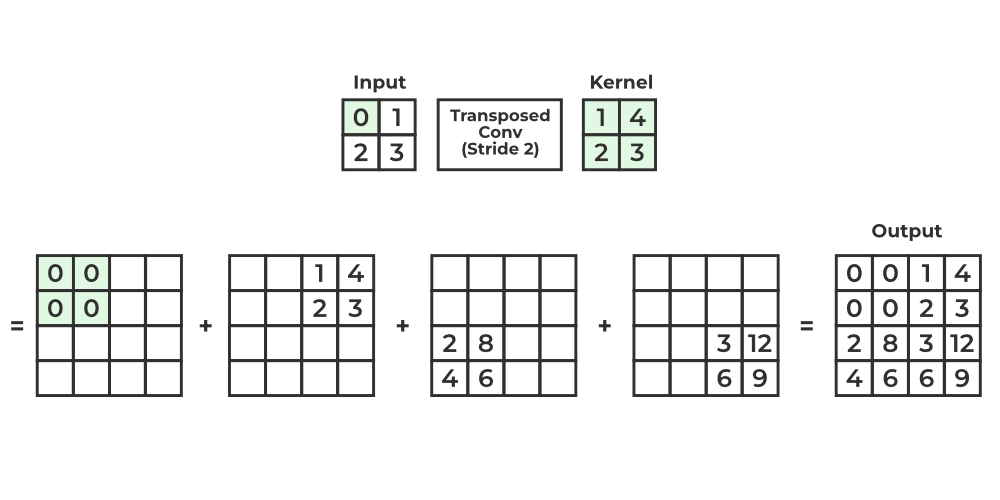
\includegraphics[width=1.0\textwidth,height=1.0\textheight,keepaspectratio]{./images/TConv.png}
\end{figure}

\begin{figure}
\centering
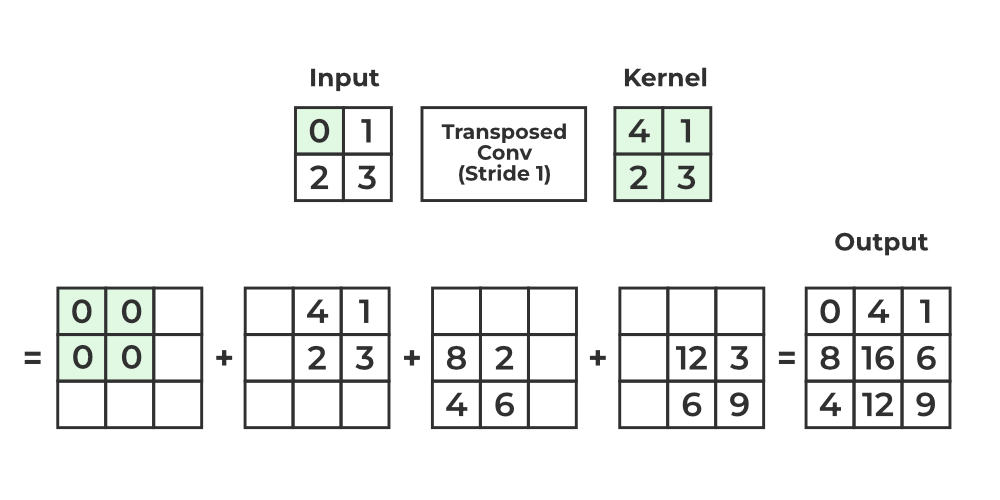
\includegraphics[width=1.0\textwidth,height=1.0\textheight,keepaspectratio]{./images/TConv2.png}
\end{figure}

\end{frame}

\begin{frame}{Mathematical Definition: Transposed Convolution}
The output \( O(x, y) \) of a transposed convolution is computed as:

\[
O(x, y) = \sum_{i,j} I(i, j) \cdot K(x - i \cdot s, y - j \cdot s)
\]

where:
\begin{itemize}
    \item \( O(x, y) \) is the output at position \( (x, y) \),
    \item \( I(i, j) \) is the input value at \( (i, j) \),
    \item \( K(x', y') \) is the kernel value at \( (x', y') \),
    \item \( s \) is the stride.
\end{itemize}
\end{frame}


\begin{frame}{Transposed Convolution Output Size Formula}

\small
\begin{equation}
\begin{aligned}
H_{\text{out}} &= (H_{\text{in}} - 1) \times \texttt{stride}[0] - 2 \times \texttt{padding}[0] \\
&\quad + \texttt{dilation}[0] \times (\texttt{kernel\_size}[0] - 1) \\
&\quad + \texttt{output\_padding}[0] + 1
\end{aligned}
\end{equation}

\begin{equation}
\begin{aligned}
W_{\text{out}} &= (W_{\text{in}} - 1) \times \texttt{stride}[1] - 2 \times \texttt{padding}[1] \\
&\quad + \texttt{dilation}[1] \times (\texttt{kernel\_size}[1] - 1) \\
&\quad + \texttt{output\_padding}[1] + 1
\end{aligned}
\end{equation}

\vspace{1em}
where:
\begin{itemize}
    \item  \( H_{\text{out}}, W_{\text{out}} \) - Output height and width.
    \item  \( H_{\text{in}}, W_{\text{in}} \) - Input height and width.
    \item  Stride - Step size of the filter movement.
    \item  Padding - Number of pixels added around the input.
    \item  Dilation - Spacing between kernel elements.
    \item  Kernel size - Size of the convolution filter.
    \item Output padding - Additional padding applied to the output.
\end{itemize}

\end{frame}

\begin{frame}{Transposed Convolution: 1D Example}


\begin{figure}
\centering
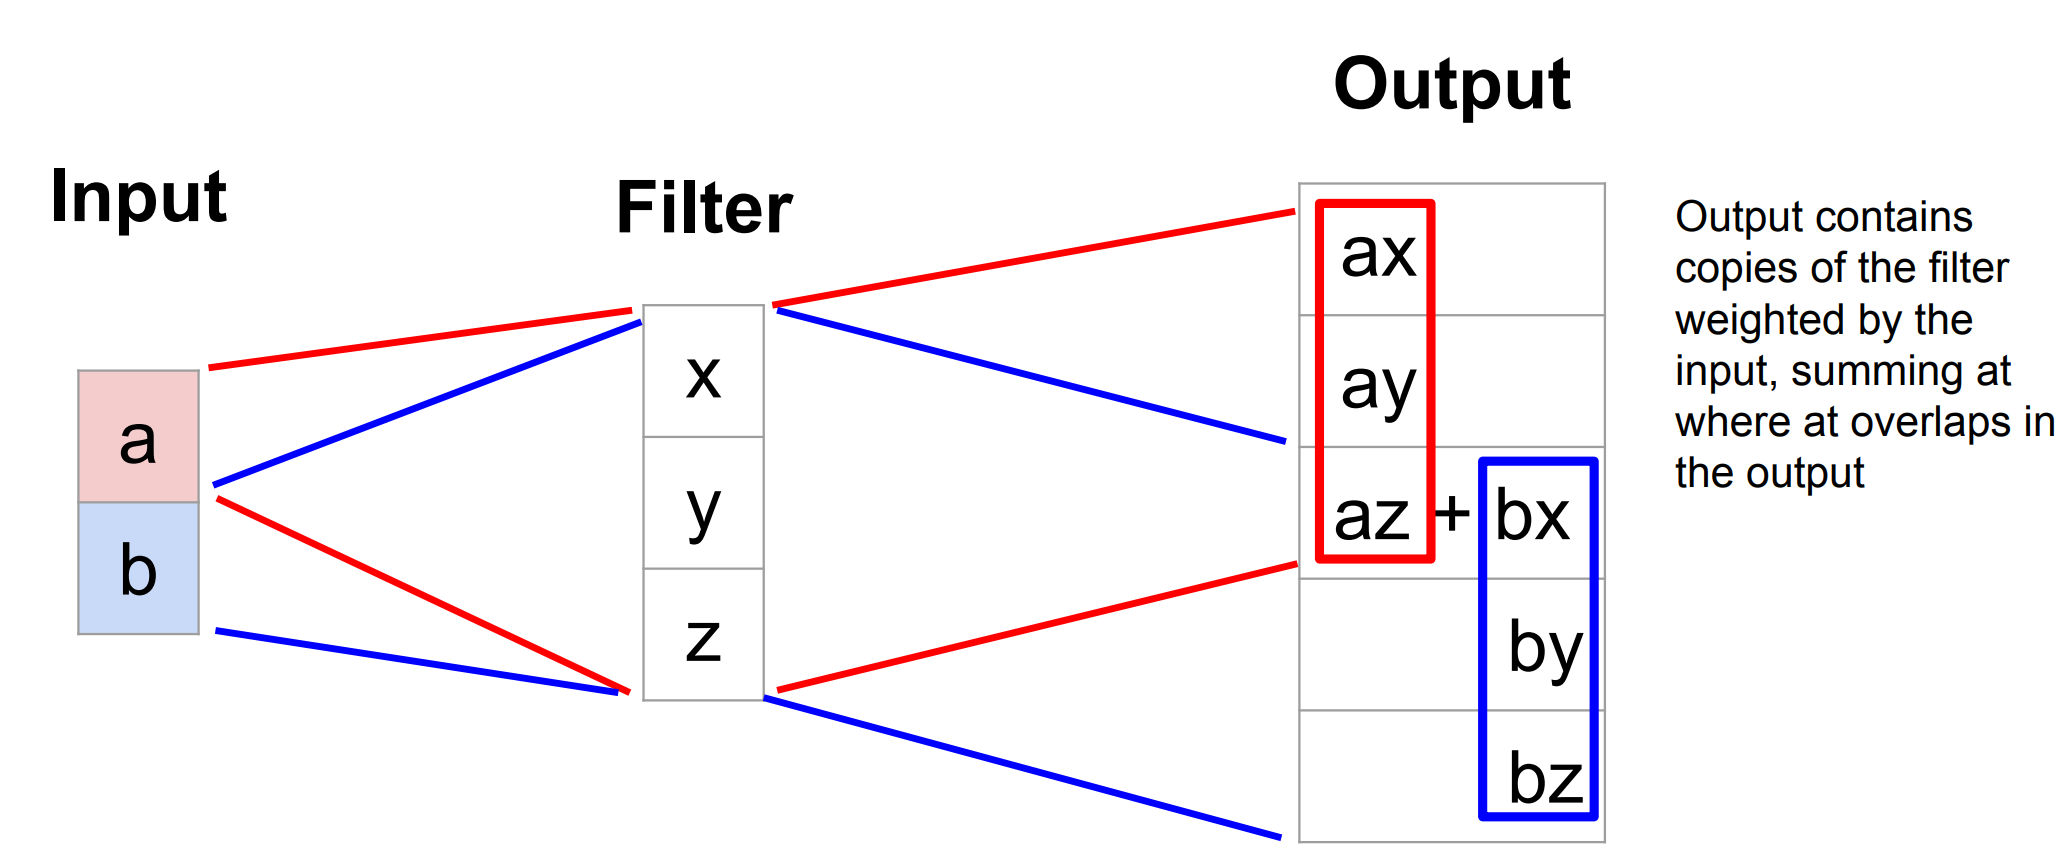
\includegraphics[width=1.0\textwidth,height=1.0\textheight,keepaspectratio]{./images/upsample_9.png}
\end{figure}


\end{frame}

\begin{frame}{Semantic Segmentation Idea: Fully Convolutional}


\begin{figure}
\centering
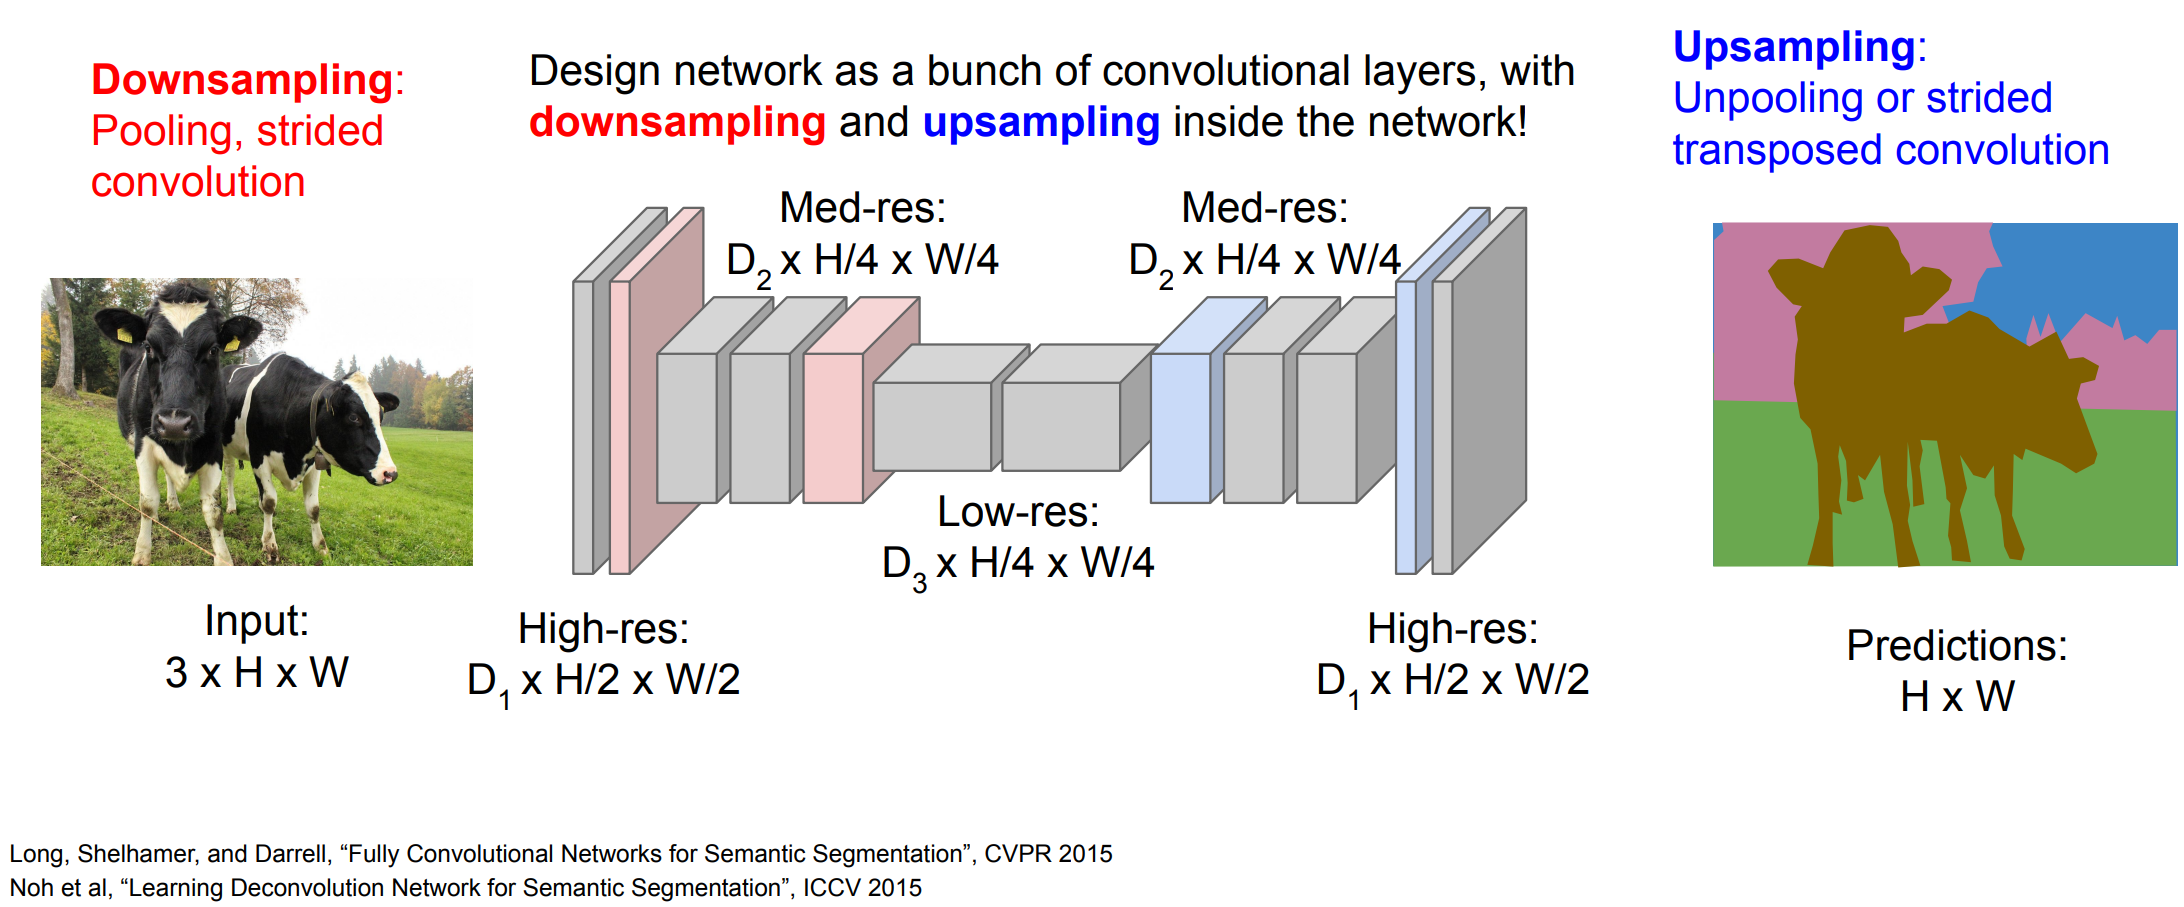
\includegraphics[width=1.0\textwidth,height=1.0\textheight,keepaspectratio]{./images/sem_11.png}
\end{figure}
\end{frame}

\begin{frame}{Can We Do Better?}
\begin{itemize}
    \item The downsampling-then-upsampling approach works well for semantic segmentation.
    \item \textbf{But... can we do better?}
        \item \textbf{Problem}: Important details and spatial information may be lost during downsampling.
    \pause
    \item \textbf{Solution}: Introduce \textbf{residual connections} to preserve spatial information.
\end{itemize}
\end{frame}

\begin{frame}{Residual Connections in Segmentation}
\begin{itemize}

        \item Directly connect features from downsampling layers to upsampling layers.
        \item Help recover lost spatial details and improve segmentation accuracy.
    \begin{figure}
    \centering
    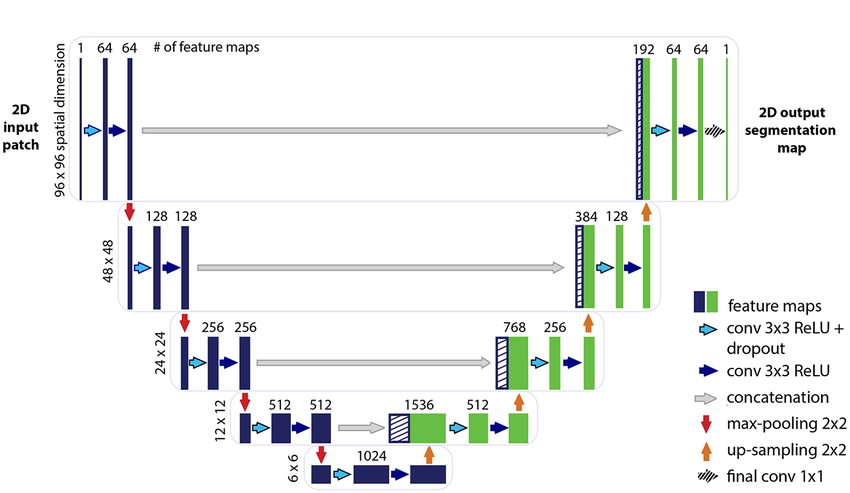
\includegraphics[width=1.0\textwidth,height=0.7\textheight,keepaspectratio]{./images/Unet.png}
    \end{figure}
    
\end{itemize}
\end{frame}

\begin{frame}{Residual Connections in Segmentation}
\begin{itemize}
    \item There are two Types of Residuals:
    \begin{itemize}
        \item \textbf{Addition:} Adds features from the encoder to the decoder \textbf{element-wise}.
        \item \textbf{Concatenation:} Concatenates features from the encoder to the decoder along the \textbf{channel dimension}.
    \end{itemize}
    \item \textbf{Which Is Better?}
    \begin{itemize}
        \item Concatenation is often better because it retains more feature information from the encoder.
        \item \textbf{Note}: technically, concatenation might be harder to implement because it requires aligning input and output shapes.
    \end{itemize}
\end{itemize}
\end{frame}

\begin{frame}{U-Net}
\begin{itemize}
    \item This architecture, with residual connections, is called \textbf{U-Net}.
    \item \textbf{Why the name?}
    \begin{itemize}
        \item The architecture resembles the shape of the letter "U".
        \item Features are downsampled in the encoder and upsampled in the decoder, with skip connections in between.
    \end{itemize}
    \item U-Net is widely used for segmentation tasks, especially in biomedical imaging.
\end{itemize}
\begin{figure}
    \centering
    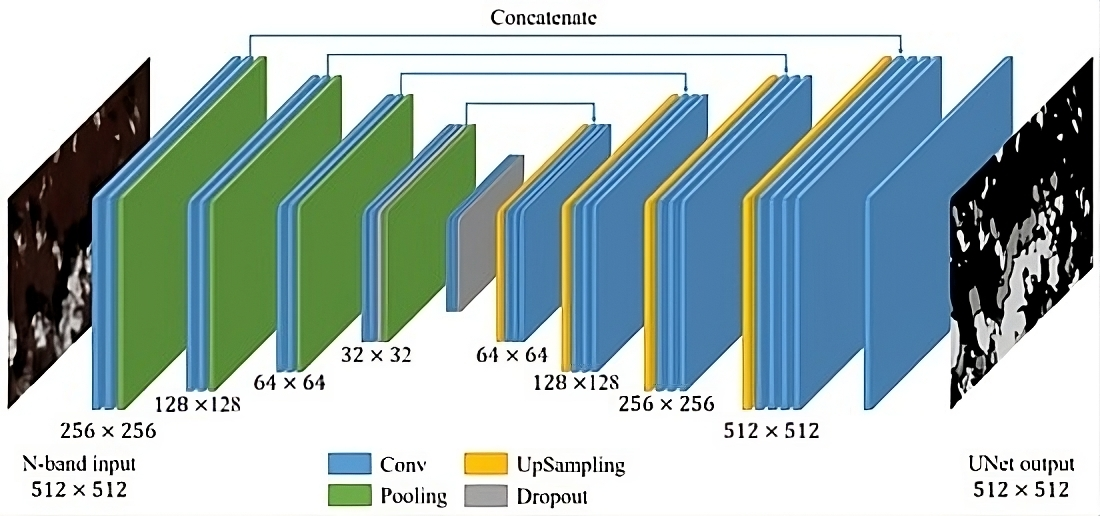
\includegraphics[width=0.75\linewidth]{images/unet2.jpeg} 
\end{figure}
\end{frame}

\begin{frame}{Using a Pretrained U-Net}
\begin{itemize}
    \item \textbf{Pretrained Encoder:}
    \begin{itemize}
        \item The encoder can use a pretrained backbone (e.g., ResNet, EfficientNet).
        \item This help utilize features learned on large datasets (e.g., ImageNet).
        \item Only the decoder is trained from scratch for segmentation-specific tasks.
    \end{itemize}
    \begin{figure}
    \centering
    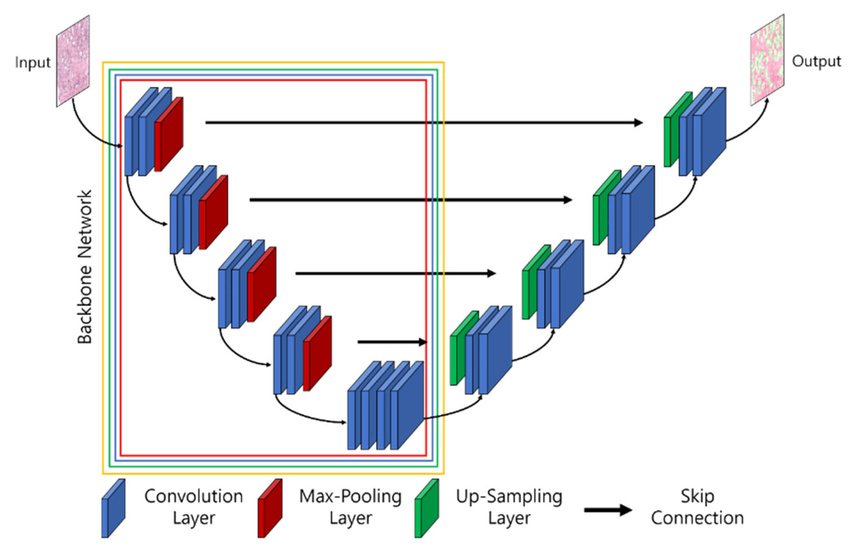
\includegraphics[width=0.75\linewidth]{images/pretrained_unet.png} 
\end{figure}
        
\end{itemize}
\end{frame}


\begin{frame}{Semantic Segmentation}
\begin{itemize}
    \item Label each pixel in the image with a category label
    \begin{figure}
    \centering
    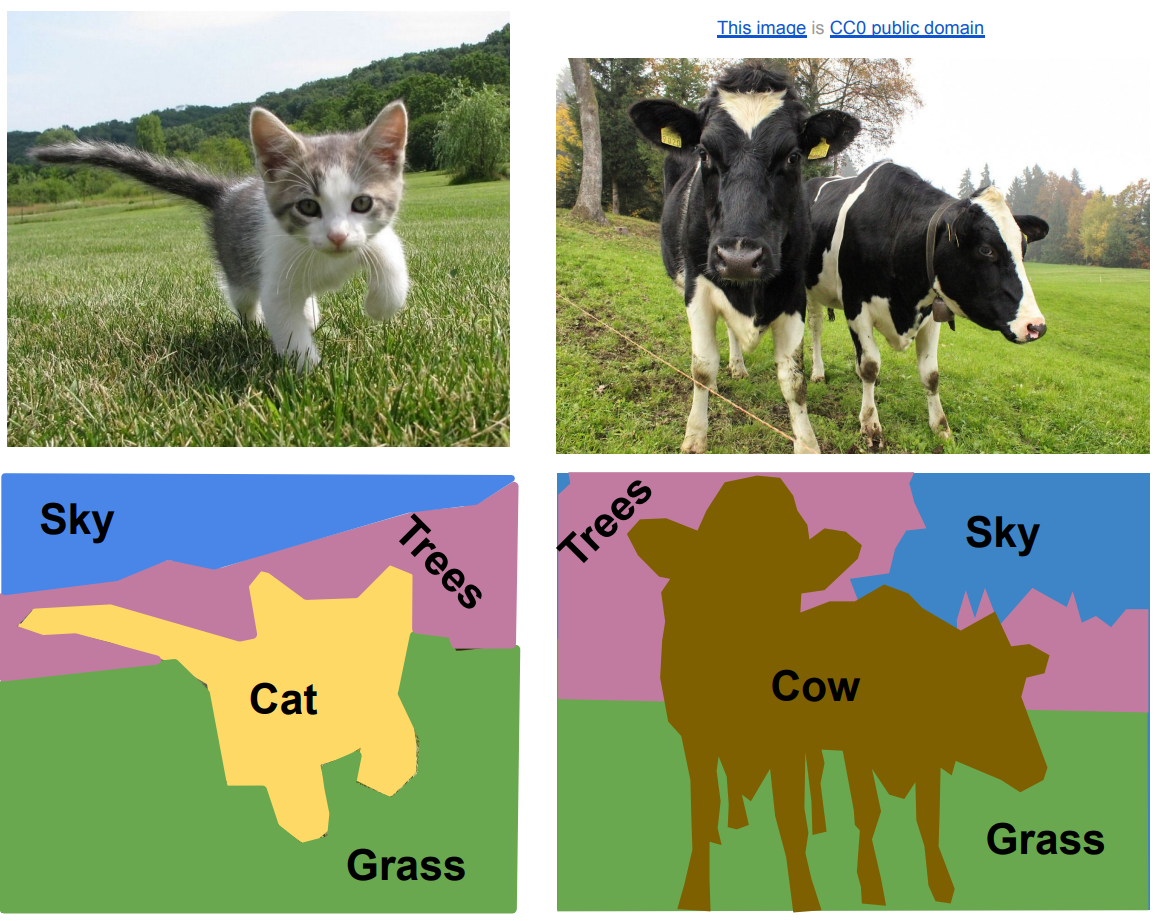
\includegraphics[width=1.0\textwidth,height=0.7\textheight,keepaspectratio]{./images/sem_12.png}
    \end{figure}
    \pause
    \item \textbf{Does not differentiate instances, only care about pixels}
\end{itemize}
    
\end{frame}

\begin{frame}{Instance Segmentation}
\begin{itemize}
    \item Separate object instances, but only things
    \begin{figure}
    \centering
    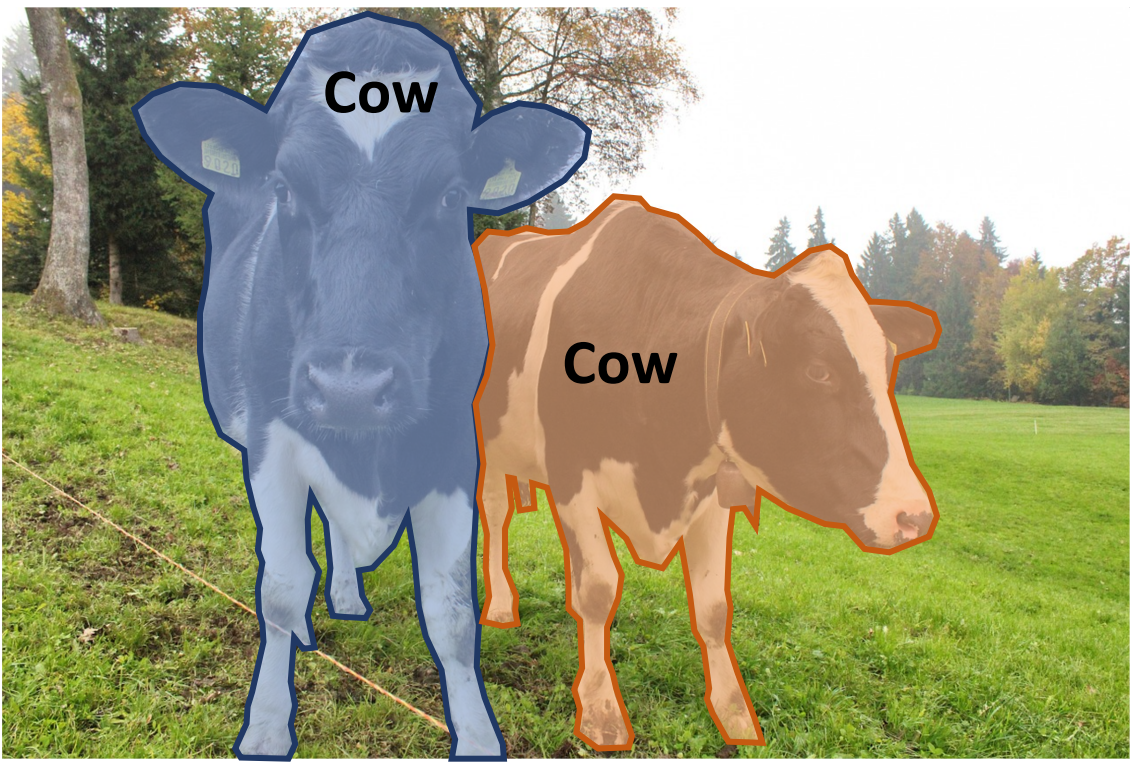
\includegraphics[width=1.0\textwidth,height=0.7\textheight,keepaspectratio]{./images/ins_4.png}
    \end{figure}
\end{itemize}
    
\end{frame}

\begin{frame}{Panoptic Segmentation}
\begin{itemize}
    \item Label all pixels in the image (both things and stuff)
    \begin{figure}
    \centering
    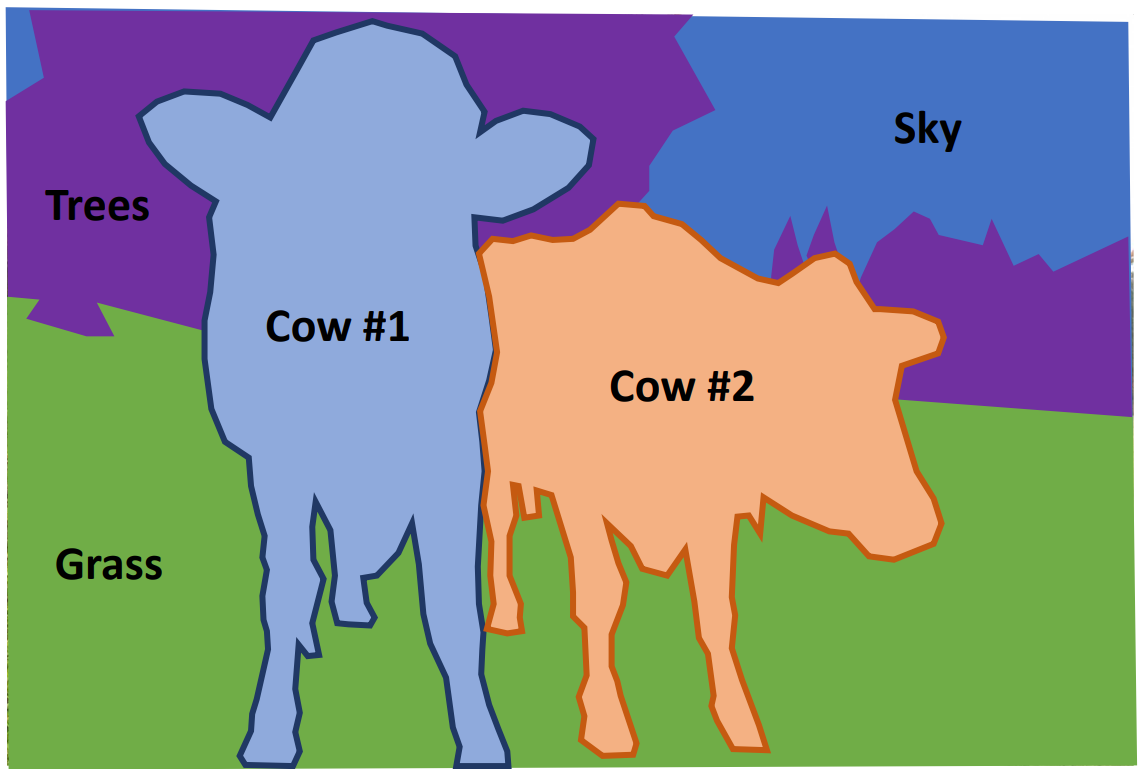
\includegraphics[width=1.0\textwidth,height=0.7\textheight,keepaspectratio]{./images/ins_10.png}
    \end{figure}
\end{itemize}
\end{frame}


\begin{frame}{References}
These slides have been adapted from
\begin{itemize}
    \item Fei-Fei Li, Yunzhu Li \& Ruohan Gao, Stanford CS231n: \href{http://cs231n.stanford.edu/index.html}{Deep Learning for Computer Vision}
    \item Assaf Shocher, Shai Bagon, Meirav Galun \& Tali Dekel, WAIC DL4CV \href{https://dl4cv.github.io/index.html}{Deep Learning for Computer Vision: Fundamentals and Applications}
    \item Justin Johnson, UMich EECS 498.008/598.008: \href{https://web.eecs.umich.edu/~justincj/teaching/eecs498/WI2022/}{Deep Learning for Computer Vision}
    % \item Sander Dieleman, Deepmind: \href{https://www.deepmind.com/learning-resources/deep-learning-lecture-series-2020}{Deep Learning Lecture Series 2020}
\end{itemize}

\end{frame}

    
\end{document}